
%*******************************************************************************
%*********************************** Second Chapter ***************************
%*******************************************************************************
%!TEX root = 0.main.tex

\section{Other samplings and other Discrete Laplacians}

In a Graph Spherical CNN we use the fact that when the sampling of the sphere is regular enough, the graph $W_{i j} = \exp {-\frac{\norm{x_i-x_j}^2}{4t}}$ is such that the corresponding graph Laplacian $\mathbf L_n^t$ has a spectrum that is close enough to the spectrum of $\triangle_{\mathbb S^2}$. In this way we can approximate a spherical convolution of a signal $f$ with a kernel $h$ with the graph convolution of the sampled signal 
$$
V\text{diag}\{h(\lambda_0), ..., h(\lambda_{n-1})\}V^T\mathbf f
$$
In Chapter 2 we showed a way to construct $\mathbf L_n^t$ that well approximates $\triangle_{\mathbb S^2}$ in the case of a regular sampling of the sphere. In this Chapter we focus on others samplings less uniform than HEALPix. The sampling that we will use for our study, very used in applications, is the so called \textit{equiangular sampling}. We observe that in this case the Heat Kernel Graph Laplacian matrix (HKGL) is not able to correctly approximate the continuous Laplace-Beltrami operator, due to the fact that the equiangular sampling samples the areas near the poles more than the area close to the equator. Figure \ref{fig:equiangular distortion} well illustrates this bad behavior of the Heat Kernel Graph Laplacian. To better show the distortion caused by the HKGL, in figure \ref{fig:equiangular distortion} the sphere was sampled with with many more samples near the poles than near the equator. The sample points are shown as the vertices of the triangulation in figure. On the left we plot one spherical harmonic $Y_\ell^m$ of degree $\ell=4$ and on the right we plot the corresponding eigenmode of the HKGL. We can see that the eigenmodes end up being artificially compressed along the equator.
\begin{wrapfigure}{r}{0.5\textwidth}
	\begin{center}
		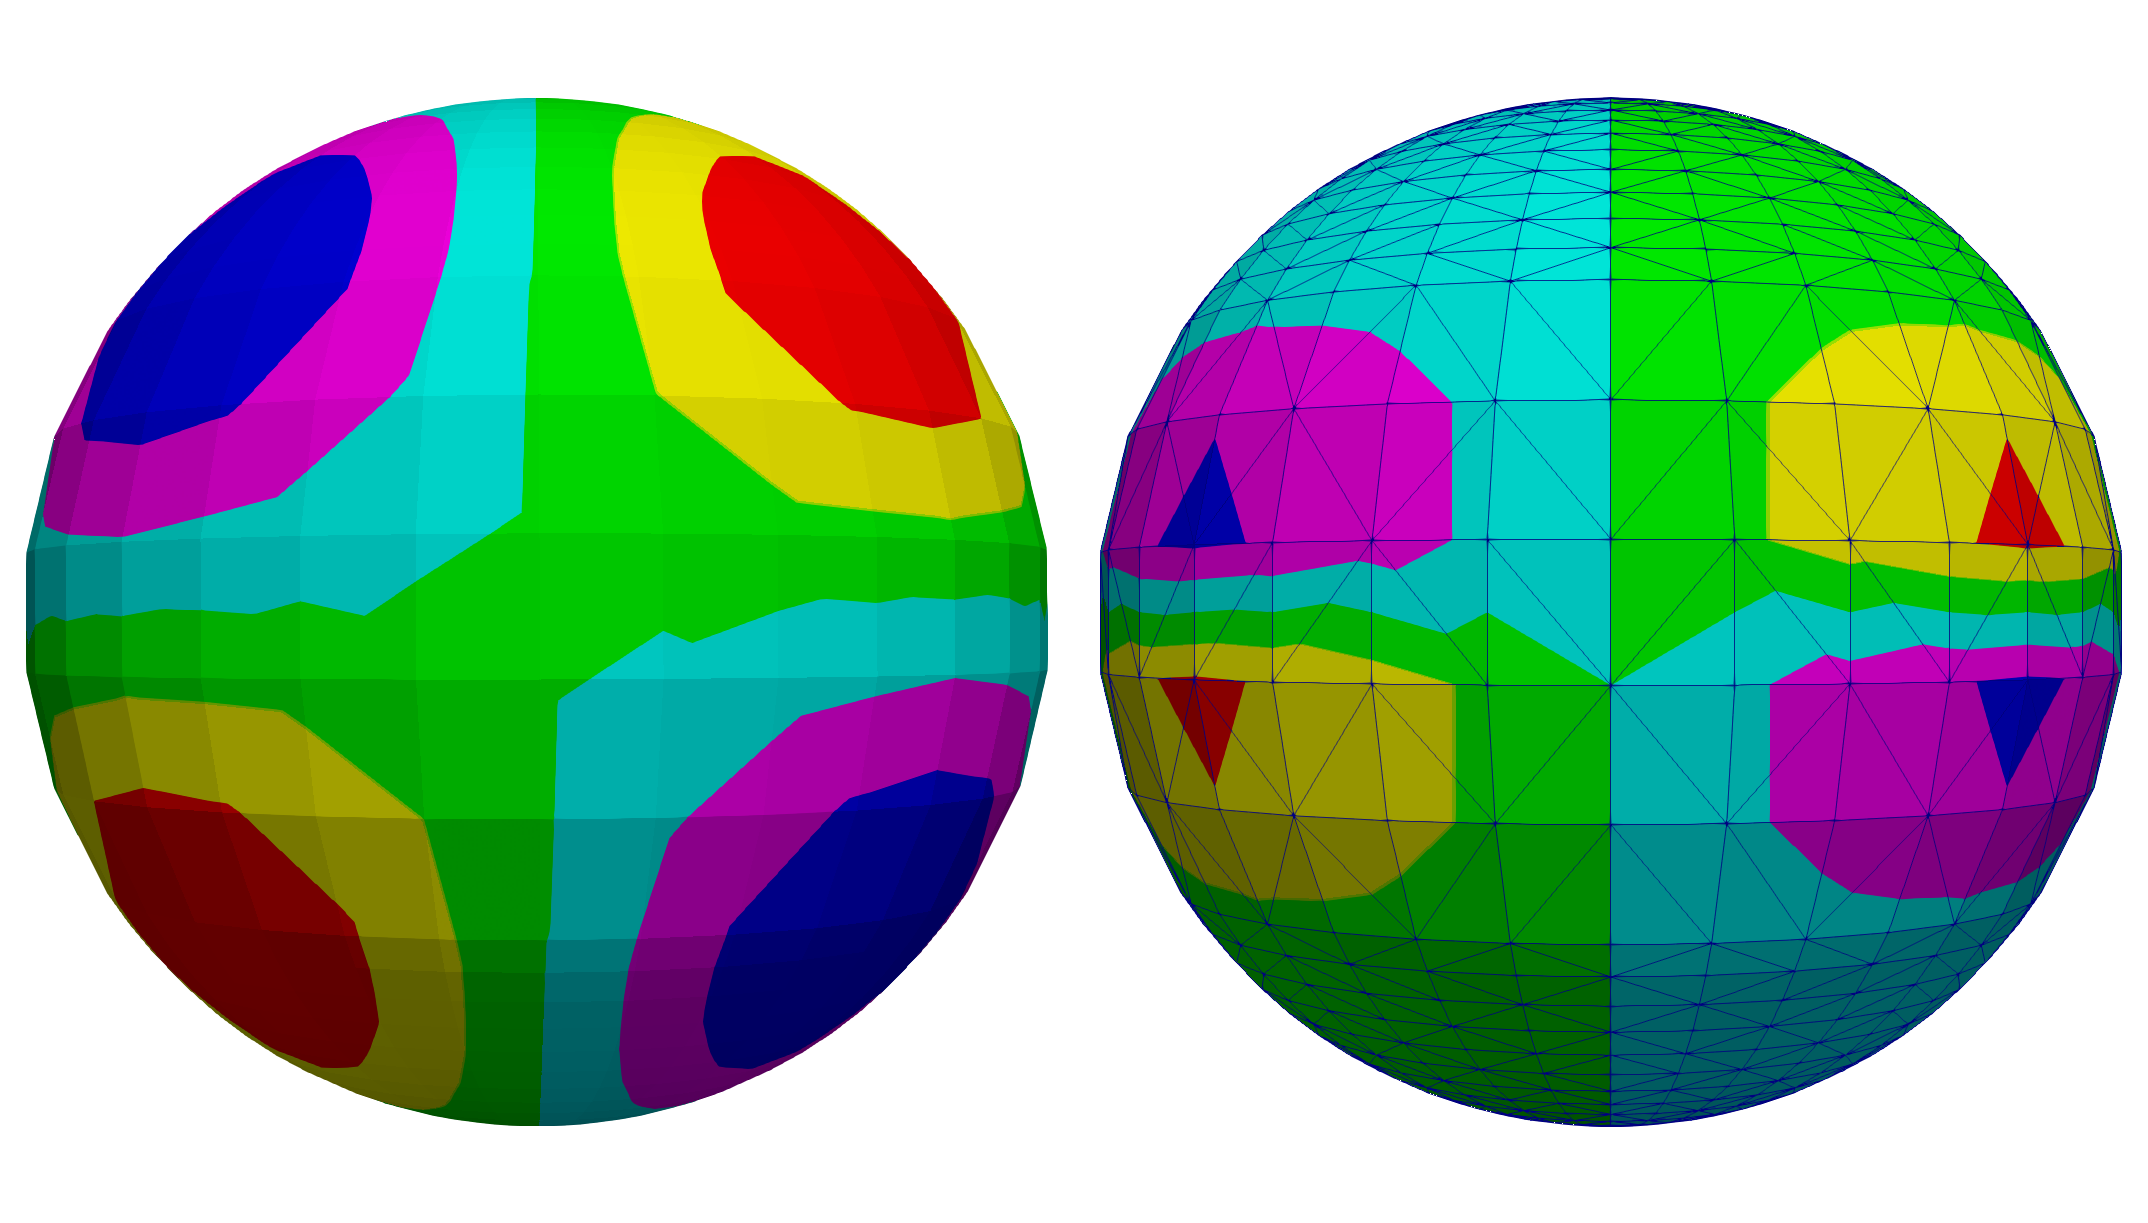
\includegraphics[width=0.5\textwidth]{../codes/04.imbalanced/img/confront_mixed.png}
	\end{center}
	\caption{\label{fig:equiangular distortion}On the left, the correct eigenmode. On the right: distortion of the eigenmode of the HKGL caused by an irregular sampling of the sphere.}
\end{wrapfigure}
The goal of this chapter is to study a way of building a discrete approximation $\mathbf L$ of the Laplace-Beltrami operator more robust to non uniform sampling than the Heat Kernel Graph Laplacian matrix $\mathbf L_n^t$ used so far.

This chapter is organized as follows: In Section \ref{sec:Chapter3: Heat Kernel Graph Laplacian on the Equiangular Sampling} we introduce the equiangular sampling and the results that we obtained with the Heat Kernel Graph Laplacian matrix. In Section \ref{sec:Chapter3: other discrete laplacians} we present a short overview of different ways of building an discrete approximation of the Laplace-Beltrami operator; in Section \ref{sec:Chapter3: Using the Finite Element Method to approximate the Laplace-Beltrami operator on a manifold} we deepen how to use the Finite Element Method (FEM) to construct a discrete approximation of $\triangle_{\mathbb S^2}$ and how it is actually capable of taking into account the non uniformity of the sampling and correct it.
\subsection{Heat Kernel Graph Laplacian on the Equiangular Sampling}
\label{sec:Chapter3: Heat Kernel Graph Laplacian on the Equiangular Sampling}

\subsubsection{The Equiangular Sampling}

Given the usual parametrization $x = x(\theta, \phi)$ of the sphere
\begin{align*}
	\mathbb{S}^{2}&=\left\{x=\left(x_{1}, x_{2}, x_{3}\right) \in \mathbb{R}^{3} :\|x\|_{\mathbb{R}^{3}}=\left(x_{1}^{2}+x_{2}^{2}+x_{3}^{2}\right)^{1 / 2}=1\right\}\\
	x_{1}&=\cos (\phi) \sin (\theta), \quad x_{2}=\sin (\phi) \sin (\theta), \quad x_{3}=\cos (\theta)
\end{align*}

Let $m\in\mathbb N$, the \textit{equiangular sampling} of bandwidth $b=2^m$ is given by 
$
x_{j k}^{(b)}=x\left(\theta_{j}^{(b)}, \phi_{k}^{(b)}\right)
$
where
\begin{align*}
	\theta_{j}^{(b)} &:=\pi \frac{j}{2 b}, \quad \phi_{k}^{(b)} :=2 \pi \frac{k}{2 b}\\
	j&=0, ..., 2b-1 \text{ and }k=0, ..., 2b-1 
\end{align*}

\begin{figure}[h]
	\centering
	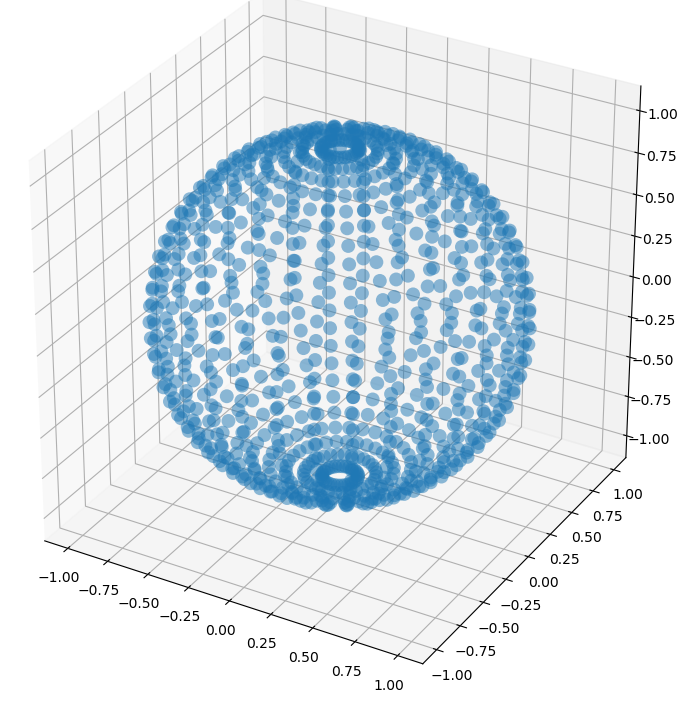
\includegraphics[width=0.5\textwidth]{figs/Chapter3/equiangular.png}
	\caption{\label{fig:equiangular sampling}Equiangular sampling with bandwidth $b=8$}
\end{figure}
One has thus $n=4b^2$ points on the sphere, where all the points $x_{0 k}^{(b)}$ correspond to the north pole for every $k=0, ..., 2b-1$. Notice also that the south pole is never sampled. In figure \ref{fig:equiangular sampling} it can also be appreciated how the area close to the poles is much more sampled that the equator. One reason for which this sampling is very used in application is the existence of the following result from \cite{Driscoll:1994:CFT:184069.184073}, that states that any band limited function can be exactly recovered from its sampled values $f\left(x_{j k}^{(b)}\right)$:
\vspace{0.5cm}
\begin{theorem}\label{theo:equiangular sampling theorem}
	Let \(l_{0} \in \mathbb{N}\) and \(m_{0} \in \mathbb{Z},\left|m_{0}\right| \leq l_{0} .\) If \(f=\sum_{l=0}^{b-1} \sum_{m=-l}^{l} \widehat{f}(l, m) Y_{l}^{m}\)
	then
	
	$$
	\begin{aligned} \widehat{f}\left(l_{0}, m_{0}\right)=& \frac{1}{4 b^{2}} \sum_{j=0}^{2 b-1} \sum_{k=0}^{2 b-1} f\left(x_{j k}^{(b)}\right) \overline{Y_{l_{0}}^{m_{0}}\left(x_{j k}^{(b)}\right)} \sin \left(\theta_{j}^{(b)}\right) \times \\ & \times \frac{4}{\pi} \sum_{l=0}^{b-1} \frac{1}{2 l+1} \sin \left((2 l+1) \theta_{j}^{(b)}\right) \end{aligned}
	$$
\end{theorem}
\vspace{0.5cm}
Theorem \ref{theo:equiangular sampling theorem} is the equivalent on the sphere of the well known Shannon's sampling theorem, that states the minimum sampling frequency at which a band limited signal $f:\mathbb R \to \mathbb R$ can be perfectly reconstructed, and is a precious tool when doing signal processing on the sphere.
\subsubsection{Heat Kernel Graph Laplacian with non uniform sampling measures}
Thanks to Theorem \ref{theo:equiangular sampling theorem}, we can compute exactly the Fourier transform of the eigenmodes of the HKGL and see how much they are aligned with the eigenspaces of the true Laplace-Beltrami operator, following the same procedure described at the beginning of Chapter 2 when introducing the same kind of plots for the HEALPix sampling. It can be appreciated how poorly aligned the eigenmodes of the HKGL are on the equiangular sampling (figure \ref{fig:equiangular sampling alignment}) compared to the ones obtained with the HEALPix sampling (\ref{fig:optimal graph})


\begin{table}[h!]
	\centering
	\begin{tabular}{ c|c } 
$b$ & $t$ \\ 
	\hline
4 & 0.5 \\ 
8 & 0.3 \\ 
16 & 0.1 \\ 
	\end{tabular}
	\caption{\label{table:equiangular kernel width}Kernel width $t$ used to construct the Heat Kernel Graph Laplacian matrix for each bandwidth $b$}
\end{table}

\begin{figure}[h!]
	\centering
	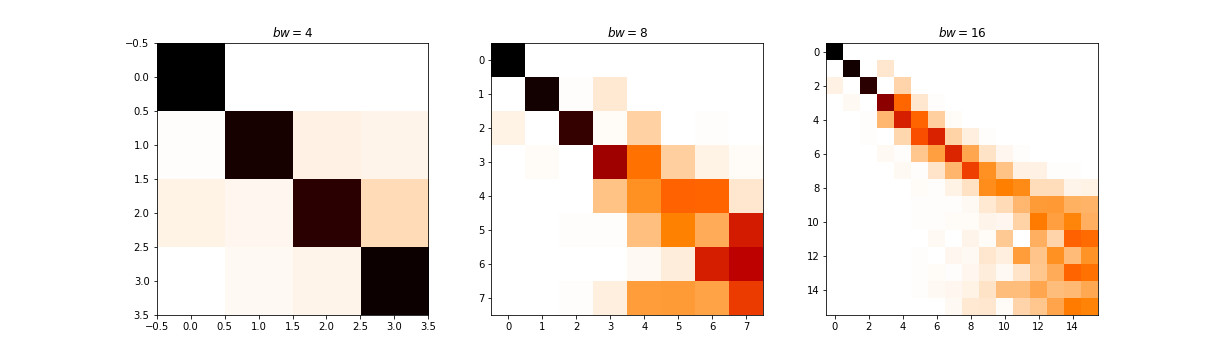
\includegraphics[width=0.9\textwidth]{../codes/02.HeatKernelGraphLaplacian/equiangular/equi_full.png}
	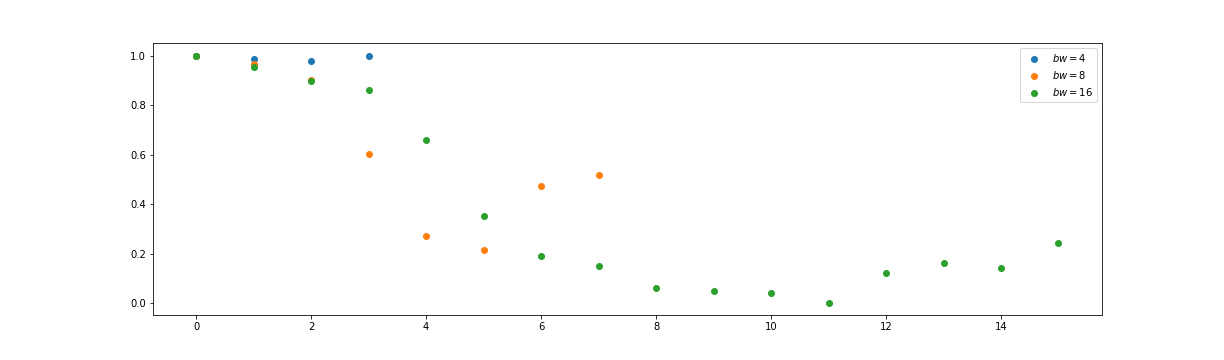
\includegraphics[width=0.9\textwidth]{../codes/02.HeatKernelGraphLaplacian/equiangular/equi_full_diagonal.png}
	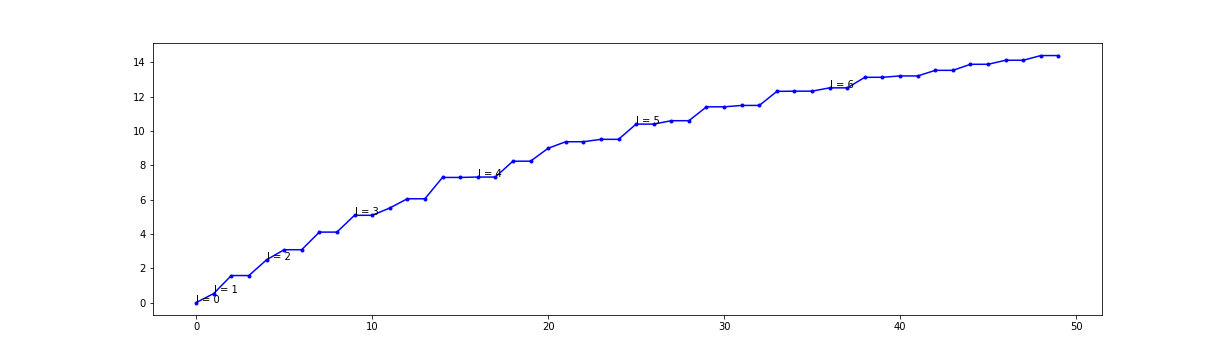
\includegraphics[width=0.9\textwidth]{../codes/02.HeatKernelGraphLaplacian/equiangular/equi_full_eigenvalues_16.png}
	\caption{\label{fig:equiangular sampling alignment}Alignment of eigenspaces of the full HKGL with respect to the true Laplace-Beltrami eigenspaces on the equiangular sampling. The kernel width for each bandwidth $bw$ are given by table \ref{table:equiangular kernel width}}
\end{figure}
The HKGL behaves badly in the case of the equiangular sampling, and does not seem to converge to $\triangle_{\mathbb S^2}$, thus making us think that the equiangular sampling does not respect the uniformity hypothesis of theorem \ref{theo:pointwise convergence in the healpix case}. The proof of Proposition 4 gives us a hint to understand the reasons behind this bad alignment of the eigenmodes. For convenience of notations define 
\begin{align*}
	\phi^{t}(x ; y):=e^{-\frac{||x-y||^2}{4t}}\left(f(y)-f(x)\right)
\end{align*}
 In order for theorem \ref{theo:pointwise convergence in the healpix case} to hold, Proposition 4 states that the Heat Kernel Graph Laplacian operator $$L_n^tf(\mathbf y)=\sum_i \frac{1}{n} \phi^{t}(\mathbf x_i ; \mathbf y)$$ must well approximate the functional approximation of the Laplace-Beltrami operator $$L^tf(\mathbf y)=\int_\mathcal M\phi^{t}(\mathbf x ; \mathbf y)d\mu(\mathbf x)$$
 where $\mu(\mathbf x)$ is the \textit{uniform probability measure} on the sphere.
The way of building the HKGL works well with a random sampling because in this case the HKGL is an \textit{unbiased estimator} of the operator $L^t$. In case of a non uniform sampling measure (as in the case of the equiangular sampling), we need to multiply the original Heat Kernel weights $W_{i j}=e^{-\frac{\norm{x_i-x_j}^2}{4t}}$ times some \textit{quadrature weights} $\alpha_i$ to create a re-weighted graph $\mathcal G'$ with adjacency matrix
$$
W'_{i j} = \alpha_i W_{i j}
$$
in order for $L_n^tf(y)$ to correctly approximate $L^tf(y)$, where $\alpha_i$ would be smaller in nodes that are in areas closer to the poles and bigger in areas closer to the equator. 

To conclude, we understood that in the case of a non uniform sampling measure the original way of Belkin et al. to construct the HKGL can not work any more, and we need an alternative way to construct a graph $W$ whose Laplacian can well approximate the Laplace Beltrami operator on $\mathbb S^2$. In the next section we present some different ways of building the discrete Laplacian matrix $\mathbf L$. Some of these do not even use the notion of graph but come from notions of Differential Geometry or Numerical Mathematics.

\subsection{Discrete Laplacians}\label{sec:Chapter3: other discrete laplacians}
Let $f$ be a sufficiently smooth function on a compact, closed infinitely differentiable manifold $\mathcal M$. The Laplacian eigenvalue problem on $\mathcal M$ is defined as 

\begin{equation}\label{eq:continous eigenvalue problem}
	\triangle_{\mathcal M}\psi = -\lambda \psi
\end{equation}


Being the Laplace-Beltrami operator self-adjoint and semi-positive definite, there exists a basis $\mathcal B=\{\psi_i\}_i$of the space $L^2(\mathcal M)$ such that $\triangle_\mathcal M \psi_i = -\lambda_i\psi_i,\ \lambda_0\leq\lambda_1\leq...,\lambda_i\leq\lambda_{i+1}...\leq+\infty$.

There's been a lot of work in trying to calculate solutions to equation \ref{eq:continous eigenvalue problem}, leading to different ways to approximate the Laplace-Beltrami operator through what we call a \textit{discrete Laplacians}. By discrete Laplacian we mean an operator $L$ that, once evaluated on a signal $f$ and on a node $x_i$ can be written as a matrix $\mathbf L$ in the following way:

\begin{equation}\label{eq:discrete laplacian}
	L f\left(\mathbf{x}_{i}\right)=\frac{1}{d_{i}} \sum_{j} w_{i j}\left(f\left(\mathbf{x}_{i}\right)-f\left(\mathbf{x}_{j}\right)\right)
\end{equation}

Note that with unit \textit{masses} $d_i=1$ we recover the same definition of Graph Laplacian. However, there are many ways to construct such matrix $\mathbf L$ that do not necessarily use a Graph perspective. Before discussing these approaches we need to introduce some basic concepts of Differential Geometry, especially the definition of mean curvature of a manifold and its link with the Laplace-Beltrami operator.

\subsubsection{Notions of Differential Geometry}

 For this short introduction to basic concepts of Differential Geometry, set the manifold $\mathcal M$ to be a differentiable, two dimensional surface embedded in $\mathbb R^3$. 
 \begin{figure}[h]
 	\centering
 	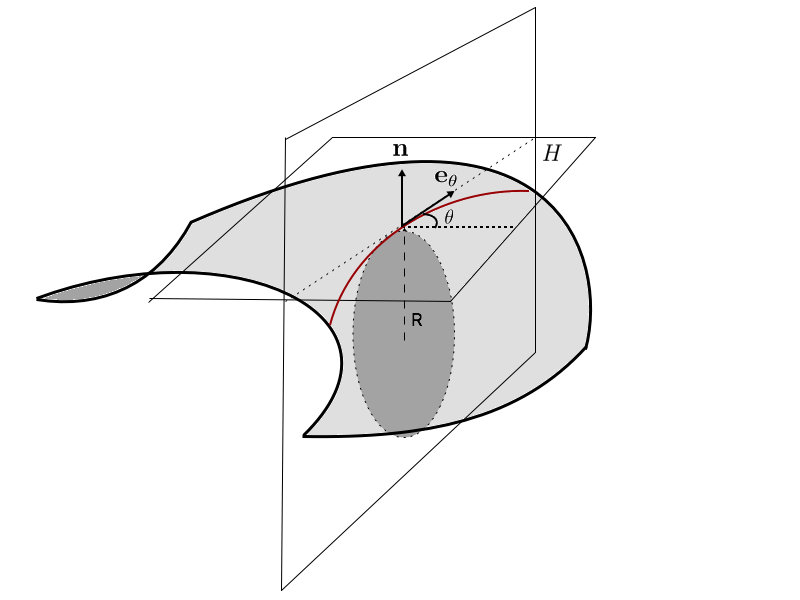
\includegraphics[width=0.5\textwidth]{figs/Chapter3/curvature.png}
 	\caption{\label{fig:curvature}Curvature normal of a manifold}
 \end{figure} 
The \textit{curvature} of a curve on a plane is defined as the inverse of the radius $R$ of the tangent circle. For each point on the manifold $\mathcal M$, define its tangent plane $H$, orthogonal to the normal vector $\mathbf n$. For every unit vector $\mathbf e_\theta$ lying on the tangent plane $H$, where $\theta$ is an angle that measures the direction on the tangent plane of $\mathbf e_\theta$, the \textit{normal curvature} $\kappa(\theta)$ is defined as the curvature of the curve that is the intersection of the manifold $\mathcal M$ and the plane containing both $\mathbf n$ and $\mathbf e_\theta$. The \textit{mean curvature} $\overline \kappa $ is defined as the average on $\theta$ of the normal curvatures:
 
 \begin{equation}\label{eq:mean curvature}
 	\overline \kappa=\frac{1}{2 \pi} \int_{0}^{2 \pi} \kappa(\theta) d \theta
 \end{equation}

It can be proved that the Laplace-Beltrami operator applied on the identity function $\mathbf x \rightarrow \mathbf x, \ \forall \mathbf x\in \mathcal M$ is directly linked to the \textit{mean curvature normal} $\overline{\kappa}\mathbf n$ by the following formula:
\begin{equation}\label{eq:laplacian and curvature}
	\triangle_\mathcal M \mathbf x  = -2\overline{\kappa}\mathbf n
\end{equation}
This equation provides us a way to approximate the Laplace-Beltrami operator through the approximation of the mean curvature normal. This fact is exploited by methods presented in the next section.



\subsubsection{Discrete Laplacians from Differential Geometry}
Desbrun et al. \cite{Desbrun1999} construct a triangulation $\mathcal T_h$ with the vertices in the sampling $x_0, x_1, ..., x_{n-1}$ approximating the manifold $\mathcal M$, and then use the following discrete expression for the \textit{discrete normal curvature} $\overline{\kappa_h} \mathbf{n}$ of the manifold $\mathcal M$:
\begin{equation}\label{eq:curvature normal}
	-\overline{\kappa_h} =\frac{1}{4 A_i} \sum_{j \in N_{1}(i)}\left(\cot \alpha_{ij}+\cot \beta_{ij}\right)\left(x_{j}-x_{i}\right)
\end{equation}


\begin{wrapfigure}{r}{0.5\textwidth}	
	\begin{center}
		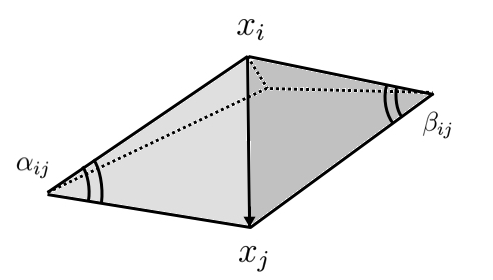
\includegraphics[width=0.3\textwidth]{figs/Chapter3/MyDesbrun.png}
		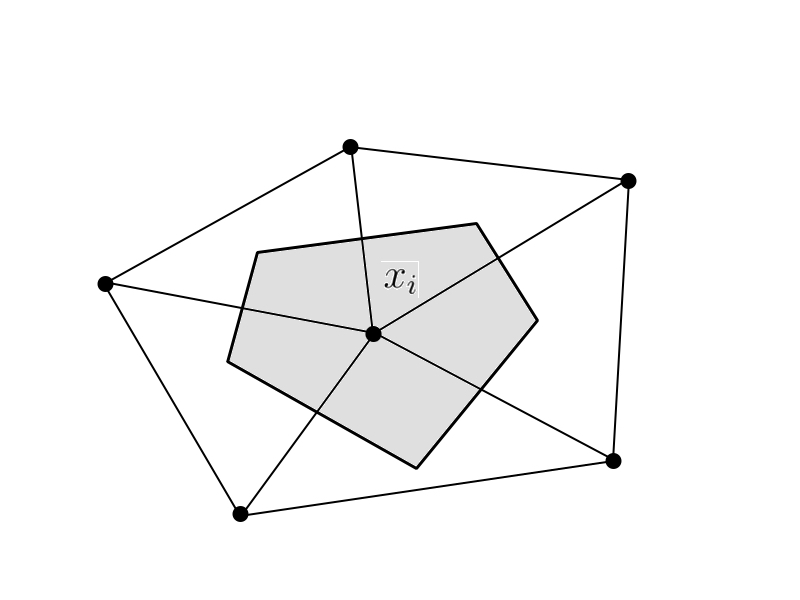
\includegraphics[width=0.3\textwidth]{figs/Chapter3/Voronoi}
	\end{center}
	\caption{\label{fig:Desbrun}One term of curvature normal formula and one Voronoi cell constructed around the node $x_i$}
\end{wrapfigure} 

where $A_i$ is the area of all the triangles of the mesh sharing the node $x_i$; $N_1(i)$ is the first ring of neighbors of the i-th node; $\alpha_{i j},\ \beta_{i j}$ are the angles of the triangles of the mesh that lie on the opposite side to the edge $(i,j)$ with respect to the node $x_i$ (Figure \ref{fig:Desbrun}). Observe that for a flat surface the discrete curvature is equal to zero $\overline{\kappa_h}=0$. This is a geometric approach that relies on the intrinsic properties of the triangulation $\mathcal T_h$ and is based on the geometric meaning of the curvature normal $\overline{\kappa}$. Using equations \ref{eq:curvature normal} and \ref{eq:laplacian and curvature} it can be shown \cite{REUTER2009381} that this approach leads to a \textit{discrete Laplacian} with masses $d_i=A_i$ where $A_i$ is the area of all the triangles of the mesh with a node in $x_i$, and weights

$$w_{i j}=\frac{\cot \left(\alpha_{i j}\right)+\cot \left(\beta_{i j}\right)}{2}$$

Meyer et al. \cite{Meyer02discretedifferential-geometry} modify the masses of Desbrun et al. and set the masses $d_i$ to be equal to $a_{V}(i)$, where \(a_{V}(i)\) is the area of the polygon obtained by joining the circumcenters of the triangles surrounding node $i$ (i.e. the Voronoi cell).


\subsubsection{A graph alternative to the HKGL for the equiangular sampling}
\begin{wrapfigure}{r}{0.5\textwidth}	
	\begin{center}
		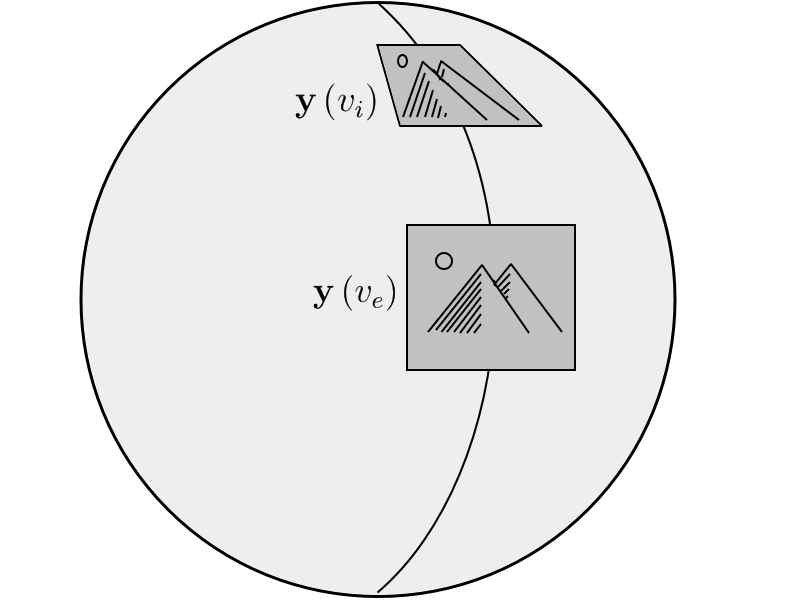
\includegraphics[width=0.9\linewidth]{figs/Chapter3/frossard2.png}
	\end{center}
	\caption{\label{fig:frossard2}Frossard et al. setting}
\end{wrapfigure} 
Frossard et al. \cite{Frossard2017GraphBasedCO} design a discrete Laplacian that is explicitly intended to work on the sphere with the equiangular sampling. They studied a way to build a graph to analyze images produced by omnidirectional cameras. In their work they assume that the image is sampled on the sphere on the equiangular sampling. They consider the set $\mathcal G$ of all the possible graphs where each node is connected only to four of its nearest neighbours (North, Sud, West, East) and propose a weighting scheme $w_{ij}$ specifically designed for the analysis of spherical signals. To design this weight scheme they minimize the difference in the response to the polynomial spectral filter $\mathcal F = \mathbf L$ evaluated on images of the same object seen at different latitudes. In other words, they solve the minimization problem

\begin{equation}\label{eq:minimization frossard}
	\min_{W\in\mathcal G} \left|\mathcal{F}\left(\mathbf{y}\left(v_{ e}\right)\right)-\mathcal{F}\left(\mathbf{y}\left(v_{ i}\right)\right)\right|
\end{equation}

for the adjacency matrix $W$, where $\mathbf y(v_i)$ is the image of the object on the sphere centered on the node $v_i$, and $\mathcal f\mathbf y(v_e)$ is the response of the filter at the node $v_e$ that lies at the same longitude of the node $v_i$ but on the equator. In their work they prove that the optimal weights solving the minimization problem \ref{eq:minimization frossard} are given by weights $w_{ij}$ inversely proportional to the Euclidean distance between nodes
\begin{equation}\label{eq:frossard weights}
	w_{ij} = \frac{1}{\norm{v_i-v_j}}
\end{equation}
This construction is interesting since it is adapted to the equiangular sampling (where the HKGL performed badly) and leads to a graph with only 4 neighbors per node, thus very sparse. Furthermore, to obtain the weights (\ref{eq:frossard weights}) every calculation was done in the \textit{spatial domain}, without any consideration about the spectral interpretation of the filter. In order to compare it to the HKGL we show the same Power Spectrum analysis in figure \ref{fig:Frossard/Khasanova graph}. It can be appreciated how this construction performs way better than the \textit{full} HKGL, having furthermore the big advantage of being naturally very sparse.
\begin{figure}[h!]
	\centering
	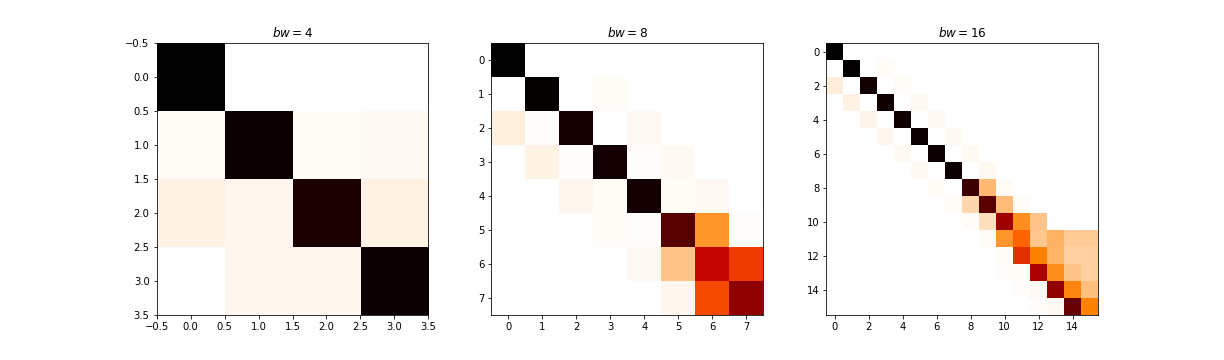
\includegraphics[width=0.9\textwidth]{../codes/02.HeatKernelGraphLaplacian/equiangular/equi_Khasanova_Frossard_full.png}
	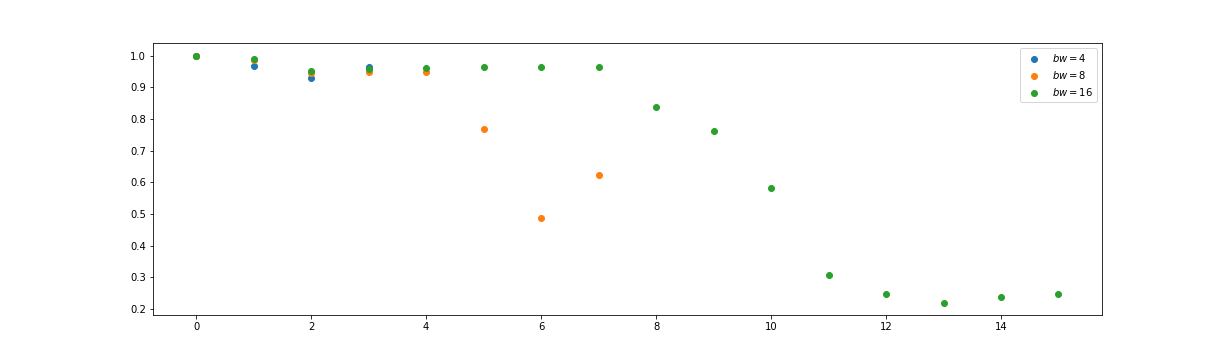
\includegraphics[width=0.9\textwidth]{../codes/02.HeatKernelGraphLaplacian/equiangular/equi_Khasanova_Frossard_full_diagonal.png}
	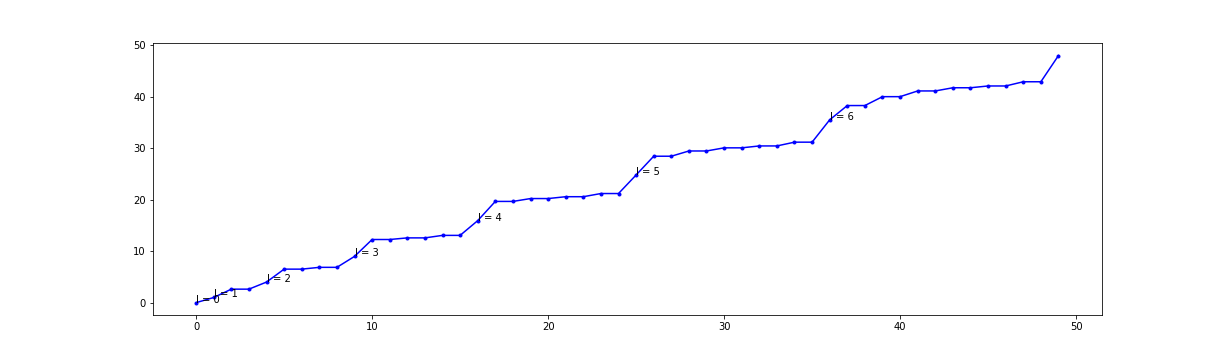
\includegraphics[width=0.9\textwidth]{../codes/02.HeatKernelGraphLaplacian/equiangular/equi_full_Khasanova_Frossard_eigenvalues_16.png}
	\caption{\label{fig:Frossard/Khasanova graph}Frossard/Khasanova graph}
\end{figure}

\subsection{The Finite Element Method approximation of the Laplace-Beltrami operator on a manifold}\label{sec:Chapter3: Using the Finite Element Method to approximate the Laplace-Beltrami operator on a manifold}
Given a differential operator $D$ and a Partial Differential Equation problem in the form
\begin{align}\label{eq:PDE}
\begin{split}
\text{Find } f(x):\Omega\in\mathbb R &\text{ such that, given }u(x):\Omega\to\mathbb R, g(x):\partial\Omega\to\mathbb R\\
Df(x)=u(x)\quad&x\in\Omega\\
f(x)=g(x)\quad &x\in\partial\Omega
\end{split}
\end{align}
the Finite Element Method (FEM) is a numerical algorithm that allows to calculate a discrete approximation of the solution $f$ through a functional discretization of the differential operator $D$. Even if in our setting we are not interested in PDE problems of the form \ref{eq:PDE}, we are interested in the FEM discretization of the differential operator $D=\Delta_{\mathbb S^2}$. In this section we provide the necessary definitions and mathematical concepts necessary to properly introduce the weak formulation of a differential problem, the Galerkin method and finally the Finite Element Method.\\
\paragraph{Banach and Hilbert spaces}
A \textit{norm} $\norm\cdot:\ X\to\mathbb R$ on a vector space $X$ is a subadditive, positive definite function such that $\norm{x+y}\leq\norm x +\norm y,\ \forall x,y\in X$ (triangle inequality). A \textit{Cauchy sequence} $(x_n)\subset X$ is a sequence such that $\forall \epsilon>0\  \exists M>0: $ $\forall i,j>M$ $ \norm{x_i-x_j}<\epsilon$. A \textit{Banach space} $(X, \norm{\cdot})$ is a normed vector space on the scalar field $F$ that is \textit{complete}, meaning that $X$ is "big enough" such that for every Cauchy sequence $(x_n)\subset X$ there exist a $x\in X$ such that $x$ is the limit of $(x_n)$ in $X$ i.e. $\norm{x_n-x}\rightarrow 0$. A \textit{basis} of $(X, \norm\cdot)$ is a minimal set of linearly independent vectors $\mathcal B \subset X$ such that every element of $X$ can be written as linear combination of the elements of $\mathcal B$. For reasons that will be clear when presenting the Galerkin method, we are interested in those particular Banach spaces where we can define a notion of orthogonality between vectors. Such Banach spaces are called \textit{Hilbert spaces}: $(X, \norm \cdot )$ is a Hilbert space when it is Banach and furthermore the norm $ \norm \cdot $ can be induced by a \textit{scalar product}: $\norm \cdot = \sqrt{\langle\cdot,\cdot\rangle}$. A scalar product is a function $\langle\cdot,\cdot\rangle: X\times X \rightarrow \mathbb F$ that is linear in the first argument, positive definite and conjugate symmetric. Through a scalar product we can define the notion of angle $\theta$ between two elements $x, y \in X$ through the following formula: 
$$
\cos \theta = \frac{\langle x, y\rangle}{\norm x \norm y}
$$ 
and in particular we can define the notion of orthogonality: two elements  $x, y \in X$ are orthogonal if and only if $\langle c, y\rangle=0$. We can now define what an \textit{orthonormal} basis of $X$ is: a basis $\mathcal B \subset X$ such that $\forall x, y \in \mathcal B, \norm x = \norm y = 1 \text{and } \langle x, y\rangle = 0$. Given an orthonormal basis $\mathcal B = \{b_i\}_{i\in I}$ we can write each vector in its \textit{Fourier series} 

\begin{equation}\label{eq:abstract fourier}
	x = \sum_{i\in I} \frac{\langle x, b_i\rangle}{\norm {x^2}}b_i
\end{equation}
If the set $I$ is countable the Hilbert space $(X, \norm\cdot)$ is called \textit{separable}. Having a countable orthonormal basis, and thus the possibility of representing each vector through its Fourier series \ref{eq:abstract fourier} enormously simplifies many problems.

\paragraph{Linear operators, functionals and bilinear forms} A \textit{linear operator} $L: X\to X$ from the Hilbert space $(X, \norm \cdot)$ to itself is a map such that $L(\alpha x + \beta y) = \alpha L x + \beta L y$. A linear operator on a Hilbert space is \textit{continuous} (or {bounded}) if $\exists M:\ |Lx|\leq Mx$. $(x, \lambda)$ are called respectively \textit{eigenvector} and \textit{eigenvalue} of the linear operator $L$ is the image of $x$ through $L$ is a rescaling of $x$ of factor $\lambda$ i.e. $Lx = \lambda x$. The operator $L$ is called \textit{self-adjoint} if $\langle Lx, y\rangle = \langle x,Ly\rangle\ \  \forall x,y \in X$. Self-adjoint operators have two important properties: their eigenvalues are real, and two eigenvectors $x, y$ associated to different eigenvalues $\lambda, \mu$ are orthogonal. Indeed 
\begin{align*}
	\langle Lx, y\rangle &= \langle x,Ly\rangle\\
	\langle \lambda x, y\rangle &= \langle x,\mu y\rangle\\
	\lambda \langle  x, y\rangle &= \mu \langle x, y\rangle
\end{align*}
that implies $ \langle  x, y\rangle = 0$. If the eigenvectors of a self-adjoint operator $L$ span the whole space $X$, than $L$ is called \textit{diagonalisable}.  A linear operator from a Hilbert space $X$ to $\mathbb R$ is called a linear \textit{functional} on $X$. A functional is bounded if $\exists M\geq 0: \ |Lx|\leq M\norm x$. The normed vector space made by the set of all linear bounded functionals on $X$ endowed with the norm $\norm L = sup_{v\in X}|Lv|/\norm v$ is called the \textit{dual} space of $X$ and is indicated with $X^\star$. An important property of linear functionals is that for every functional $L\in X^\star$, there exists a unique vector $u\in X$ such that
$$Lv = \langle u, v\rangle\quad \forall v\in X$$ 

A \textit{bilinear form} on the vector space $X$ is a map $a(\cdot, \cdot): X\times X\to F$ that is linear with respect to both arguments. It is said to be \textit{strongly coercive} if $\exists\alpha>0:\ |a(x, x)|\geq \alpha \norm {x}^2$, and \textit{bounded} if $\exists M>0:\ |a(x, y)|\leq M \norm x \norm y$.

\paragraph{The Lax-Milgram theorem}
Before introducing the Galerkin method the last thing to do is to state the Lax-Milgram theorem, theorem that is the foundation of the FEM formulation.
\vspace{0.5cm}
\begin{theorem}[Lax-Milgram]
	If \(a(\cdot, \cdot)\) is a bounded and strongly coercive bilinear form on the Hilbert space \(X\),  $L\in X^\star$ is a linear bounded functional on $X$, there exist a unique solution $f$ to the following problem:
	\begin{equation}\label{eq:variational abstract problem}
	\text{Find }f\in X\text{ such that } a(f, v)=Lv \text{ for all } v \in X
	\end{equation}
	For such \(f\) one has \(\|f\| \leq \frac{1}{\alpha}\norm L\) where \(\alpha>0\) is the coercive constant \(a(v, v) \geq \alpha\norm v^{2} \forall v \in X.\)
\end{theorem} 
\vspace{0.5cm}
The Finite Element Method takes a PDE problem in strong form \ref{eq:PDE}, reformulates it in the equivalent \textit{weak form} \ref{eq:variational abstract problem} through suitable definitions of $X, a(\cdot, cdot), L$ and finally solves it through polynomial interpolation.
\subsubsection{Weak formulation of a PDE and Galerkin Method}

Galerkin's method is a method to approximate the solution $f$ of an infinite dimensional problem of the form \ref{eq:variational abstract problem} with the solution $f_h$ of a finite dimensional problem. Our goal is now to explain how to write a differential problem like 
\begin{align}\label{eq:strong form}
\begin{split}
&\text{Given a regular domain }\Omega\subset\mathbb R^2\text{ and } u\in C(\Omega)\text{, find }f\in C^2(\Omega) \text{ such that}\\
&\begin{cases}
-\partial_{x_1x_1}f(\mathbf x) - \partial_{x_2x_2}f(\mathbf x) = u(\mathbf x) & \mathbf x \in \Omega\\
f(\mathbf x) =  0& \mathbf x \in \partial \Omega
\end{cases}
\end{split}
\end{align}
in the form \ref{eq:variational abstract problem}. Let's multiply the differential equation times a sufficiently regular function $v$ that vanishes on $\partial \Omega$ and integrate on $\Omega$. We obtain
\begin{align}
\begin{cases}
-\int_{\mathbb S^2}\Delta f(\mathbf x)v(\mathbf x)d\mathbf x =\int_{\mathbb S^2} u(\mathbf x)v(\mathbf x)d\mathbf x &\quad \mathbf x \in \Omega\\
f(\mathbf x) =  0&\quad \mathbf x \in \partial \Omega
\end{cases}	
\end{align}
 Since the contribution of both $f$ and $v$ on the border $\partial \Omega$ is zero, $\int_{\partial \Omega}\nabla f \cdot \mathbf nv d\sigma=0$ and integrating by parts we get

\begin{equation}\label{eq:int by parts}
	\int_\Omega \nabla f(\mathbf x)\cdot\nabla v(\mathbf x) d\mathbf x = \int_\Omega  u(\mathbf x)\cdot v(\mathbf x)d\mathbf x
\end{equation}

By defining $a(f, v):=	\int_\Omega \nabla f(\mathbf x)\cdot\nabla v(\mathbf x) d\mathbf x $ and $Lv := \int_\Omega  u(\mathbf x)\cdot v(\mathbf x)d\mathbf x$ problem \ref{eq:int by parts} can be written in the form of equation \ref{eq:variational abstract problem}. It remains to choose a Hilbert space $(X, \langle\cdot,\cdot\rangle_X)$ such that (i) $X$ it is "big enough" to include those functions such that all the integrals and derivatives in the problem \ref{eq:int by parts} is well defined. This means that $X$ must include those functions $f$ such that $f, \nabla f$ are in $L^2(\Omega)$ and has to be \textit{complete} with respect to the norm induced by the scalar product $\langle\cdot,\cdot\rangle_X$. At the same time $X$ must be (ii) "small enough" to include only those functions that are vanish on the boundary of $\Omega$. and (iii) the hypothesis of the Lax-Milgram theorem are satisfied, i.e. $a(\cdot, \cdot)$ is actually bounded and coercive and $L$ is a bounded and linear. It turns out that such an Hilbert space exists: it is called $H^1_0(\Omega)$, it contains all the functions $v$ such that $v\in L^2(\Omega), \nabla v\in L^2(\Omega)$ and it is endowed with the scalar product 
$$
\langle u, v\rangle_{H^1_0(\Omega)} = \int_\Omega u(\mathbf x)v(\mathbf x)d\mathbf x + \int_\Omega\nabla u(\mathbf x)\cdot \nabla v(\mathbf x) d\mathbf x
$$
$H^1_0$ contains only those functions that vanish on $\delta \Omega$ i.e. $f\in H^1_0(\Omega)\cap C(\Omega) \implies \left.f(\mathbf x)\right|_{\partial\Omega}=0$. This means that thanks to Lax-Milgram theorem the problem

\begin{equation}\label{eq:final variational form}
\begin{split}
	&\text{Given }u\in L^2(\Omega)\text{ find }f\in H^1_0(\Omega)\text{ such that }\\
	&\int_\Omega \nabla f(\mathbf x)\cdot\nabla v(\mathbf x) d\mathbf x = \int_\Omega  u(\mathbf x)\cdot v(\mathbf x)d\mathbf x\quad \forall v\in H^1_0(\Omega)
\end{split}
\end{equation}

\textit{has one and only one solution in} $H^1_0(\Omega)$. However, to have this result (existence and uniqueness of the solution) we had to pay the price of looking for the solution $f$ in $H^1_0(\Omega)$, a much bigger space than  $C^2(\Omega)$ that we had in the original, strong form of the problem. This means that our solution $f\in H^1_0(\Omega)$ to the problem (\ref{eq:final variational form}) could not be a solution to problem (\ref{eq:strong form}), because it could be not regular enough and the second derivative $\Delta f$ could not exist! Fortunately there are regularity results - that we omit here - that assure that if the forcing term $u$ is regular enough, than also the solution $f$ will be regular and thus the two formulations - strong and weak - of the problem are actually equivalent, and thus solving \ref{eq:final variational form} eventually leads to solving \ref{eq:strong form}.

Now that we know that a solution exists, we need to compute it! Computing it analytically is often impossible; Galerkin's method in a mathematical tool provide us a way to compute an approximation of the solution $f$. Take the weak problem \ref{eq:variational abstract problem}, but restrict the ambient space to be a finite dimensional subspace of $X$, say $V_h = \text{span}\{\phi_0, ..., \phi_{n-1}\}$. We write thus the Galerkin problem
\vspace{0.5cm}

\begin{equation}\label{eq:Galerkin problem}
		\text{Find }f_h\in V_h\text{ such that } a(f_h, v_h)=\langle u_h, v_h\rangle \text{ for all } u_h \in V_h
\end{equation}
\vspace{0.5cm}

The key property of the Galerkin method is that the error $f-f_h$ is orthogonal to $V_h$; thus by choosing a sequence of finite dimensional spaces that fill the original space $X$, we can get as close as we want to the continuous solution $f$.
To solve equation \ref{eq:Galerkin problem} we write $f_h, u_h, v$ as linear combinations of the basis $\{\phi_0, ..., \phi_{n-1}\}$
\begin{equation}\label{eq:basis functions}
	\begin{cases}
	f_h = f_0\phi_0 +  f_1\phi_1 + ...  f_{n-1}\phi_{n-1}\\
	u_h = u_0\phi_0 +  u_1\phi_1 + ...  u_{n-1}\phi_{n-1}\\
	v_h = v_0\phi_0 +  v_1\phi_1 + ...  v_{n-1}\phi_{n-1}
	\end{cases}
\end{equation}
 thus obtaining by linearity of the bilinear form and of the scalar product a linear system of equations in the $n$ coordinates of $f_h$
\begin{equation}\label{eq:Galerkin problem in the basis functions}
\text{Find }\mathbf f\in\mathbb R^n\text{ such that } \sum_{j=0}^{n-1}a(\phi_i, \phi_j)f_j=\sum_{j=0}^{n-1}\langle \phi_i, \phi_j\rangle u_j \text{ for all } i=0, ... n-1
\end{equation}

Defining the \textit{stiffness matrix} $(A)_{ij} = a(\phi_i, \phi_j)$ and the \textit{mass matrix} $(B)_{ij} = \langle \phi_i, \phi_j\rangle$ we can rewrite problem \ref{eq:Galerkin problem in the basis functions} in the following algebraic form
\begin{equation}\label{eq:Galerkin algebraic}
\text{Find }\mathbf f\in\mathbb R^n\text{ such that } A\mathbf f = B \mathbf u
\end{equation}
where $\mathbf f, \mathbf u$ are the vectors of coordinates of $f_h, u_h$ with respect to the basis $(\phi_i)$. 
\vspace{0.5cm}
\begin{remark}
	 If the basis functions $\phi_i$ are orthonormal, then the mass matrix $B$ equals to the identity matrix. Furthermore, the scalar product in the space $V_h$ of two functions $u_h, v_h$ is equal to the dot product defined by the mass matrix $B$ in $\mathbb R^n$ of the coordinate vectors
	\begin{equation}\label{eq:dot product}
	\langle u_h, v_h\rangle = \mathbf u^T B \mathbf v
	\end{equation}
	The Galerkin method \ref{eq:Galerkin problem} is well posed by a straight-forward application of the Lax-Milgram theorem, and thus also the system \ref{eq:Galerkin algebraic} admits one and only one solution.
\end{remark}

 \subsubsection{The Finite Element Method}
 
  The Finite Element Method is a technique that let us construct a particular subspace $V_h$ in (\ref{eq:Galerkin problem}) through polynomial interpolation. Let's refer again to the problem \ref{eq:strong form} defined on the domain $\Omega\subset\mathbb R^2$ in figure \ref{fig:omega and mesh}. 
 \paragraph{Approximation of the domain $\Omega$}
\begin{figure}[h]
	\centering
	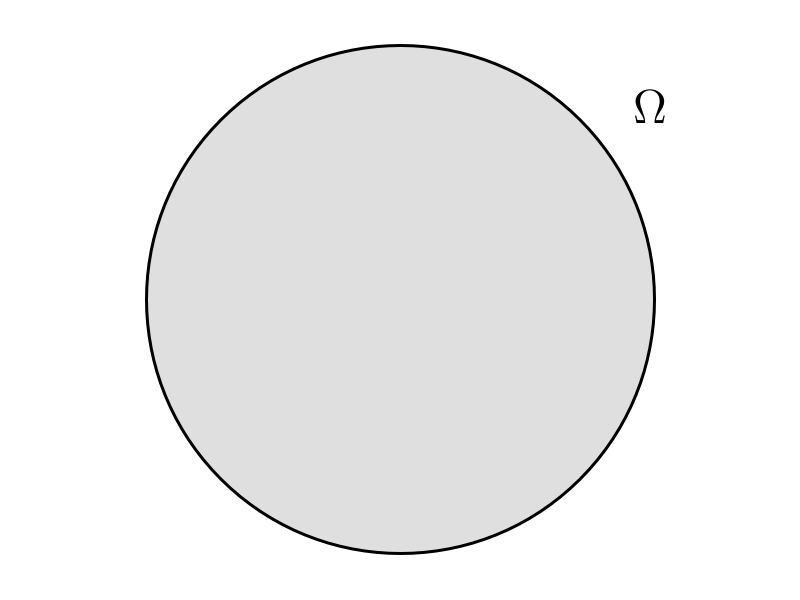
\includegraphics[width=0.4\textwidth]{figs/Chapter3/omega.png}
	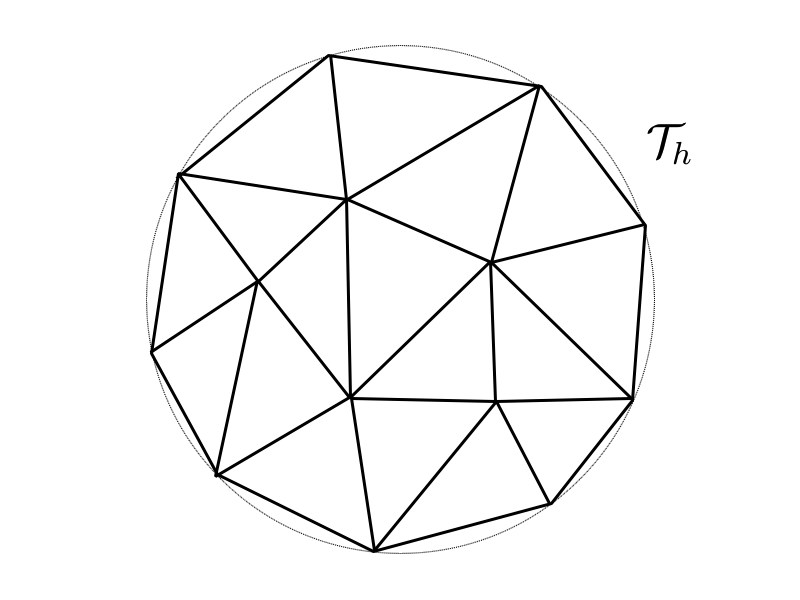
\includegraphics[width=0.4\textwidth]{figs/Chapter3/mesh.png}
	\caption{\label{fig:omega and mesh}The domain $\Omega$ and its approximation $\mathcal T_h$}
\end{figure}
First we need to construct a discretization of the continuous domain $\Omega$. In this example we take the triangulation in figure \ref{fig:omega and mesh} $\mathcal T_h = \left\{\tau_{k} : 1 \leq k \leq q\right\}$, where $h\in\mathbb R$ is a parameter such that every edge of the triangles $\tau_k\in\mathcal T_h$ is smaller than $h$. $\mathcal T_h$ is such that 
\begin{itemize}
	\item The elements \(\tau \in \mathcal{T}_h\) are closed subsets of \(\Omega\) with pairwise disjoint interior and \({\Omega}_h=\bigcup_{\tau \in \mathcal{T}_h} \tau\)
	\item The triangulation \(\mathcal{T}_h\) has no hanging vertices.
\end{itemize}
\begin{figure}
	\begin{center}
		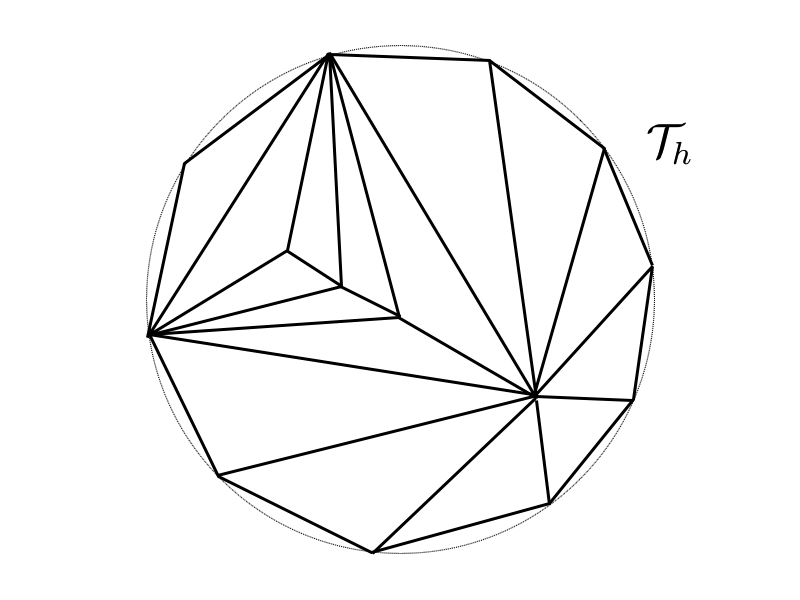
\includegraphics[width=0.4\textwidth]{figs/Chapter3/badmesh.png}
	\end{center}
	\caption{\label{fig:bad mesh}A bad quality mesh}
\end{figure}
It's clear that by discretizing the continuous domain $\Omega$ we introduce a first source of errors in the method; however for simplicity we won't take this into account in the next discussion, and we will identify the domain $\Omega$ with the domain $\Omega_h$covered by $\mathcal T_h$. The quality of the \textit{mesh} $\mathcal T_h$ is important for a good solution; a good quality mesh should avoid triangles with extreme angles and every triangle of $\mathcal T_h$ should look like as much as possible to an equilateral triangle. In figure \ref{fig:bad mesh} we see an example of a bad quality mesh: its triangles look very stretched; there are vertices that are shared by many triangles and vertices that are shared by very few. In figure \ref{fig:omega and mesh} we see a better mesh: there are no stretched triangles, and every node is shared by an almost constant number of triangles.

\paragraph{Choosing the subspace $V_h$ and the basis functions $\phi_i$}
\begin{wrapfigure}{r}{0.5\textwidth}
	\begin{center}
		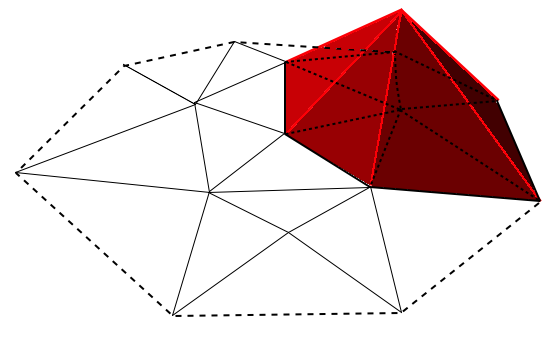
\includegraphics[width=0.4\textwidth]{figs/Chapter3/basisfunction.png}
	\end{center}
	\caption{\label{fig:basis function}Basis function of the space $X^{1}_h$}
\end{wrapfigure}
Once chosen our domain discretization $\mathcal T_h$, we need to choose the space $V_h$ we want to use for our Galerkin problem. Define 
$$X_h^{1}=\{v_h: v_h\in C(\Omega): \left.v_h\right|_{\tau}\in\mathbb P^1\  \forall \tau\in \mathcal T_h\}$$
to be the space of all the continuous, piecewise linear functions on $\Omega$. A reasonable choice for $V_h$ is the space $X_h^{1,0}\subset H_0^1(\Omega)$ of the functions of $X_h^1$ that vanish on $\partial \mathcal T_h$
$$
X_h^{1,0}=\{v_h: v_h\in C(\Omega): \left.v_h\right|_{\tau}\in\mathbb P^1\  \forall \tau\in \mathcal T_h, \left.v_h\right|_{\partial\Omega}=0\}
$$ 
Since for the functions in $X_h^1$ the number of degrees of freedom is the same of the number of nodes of the mesh $n$, we need  $n$ basis functions $\phi_i, i=0,...,n-1$ to fully describe $X_h^{1}$. The most natural choice for $\phi_i$ is the following: $\phi_i$ is defined as the continuous piecewise linear function such that 
$$
\phi_i(x_j) = \delta_{ij}\quad i=0,...,n-1
$$
The support of $\phi_i$, i.e. the subset of $\mathcal T_h$ where $\phi_i$ is not zero is made by all the triangles sharing the i-th node. An example is shown in figure \ref{fig:basis function}. To obtain a basis for the smaller space $X_h^{1,0}\subset X_h^{1}$ we just not take into account those $\phi_i$ that assume positive values on the nodes belonging to the border $\partial\Omega$. 

\vspace{0.5cm}
\begin{remark}
	For a function $v_h \in X^1_h,\ v_h = v_0 \phi_0 +...  v_n \phi_n$ the coefficient $v_i$ is equal to the function $v_h$ evaluated in the $i-th$ node 
	\begin{equation}\label{eq:dof and values}
		v_i = v_h(\mathbf x_i)
	\end{equation}
\end{remark}\vspace{0.5cm}

Other choices for $V_h$ are possible; another common choice is the space $X_h^{2}$ that is the space of all the piecewise second-order polynomials. In this case, since every second order polynomial in $\mathbb R^2$ has 6 degrees of freedom per each triangle $\tau_k$, meaning that we need to know its values in at least 6 different points on the triangle $\tau_k$ to uniquely identify it, the dimension of the space will grow (figure \ref{fig:elements}). A bigger space means that the approximation $f_h$ will be better, but we'll need more basis functions to define and thus it will result in a bigger linear system \ref{eq:Galerkin algebraic} and higher computational costs.
\begin{figure}[h!]
	\begin{center}
		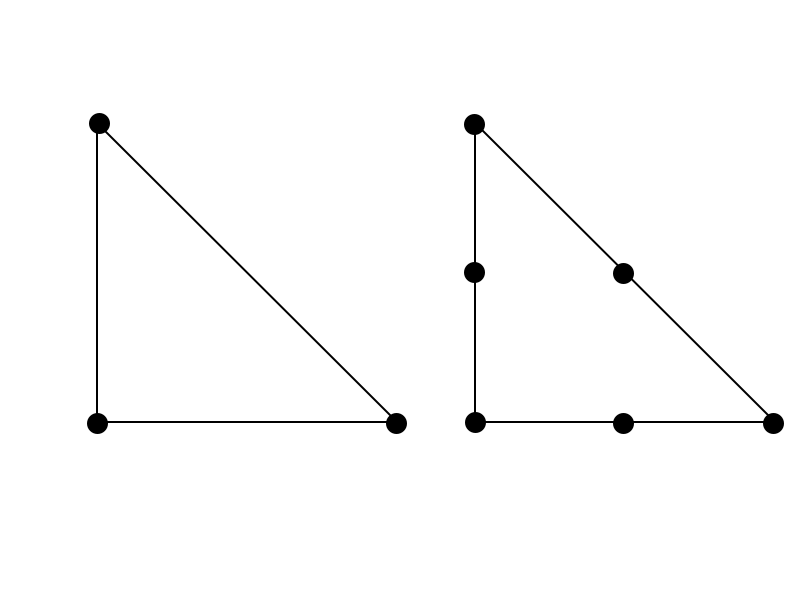
\includegraphics[width=0.4\textwidth]{figs/Chapter3/elemntsP1P2.png}
	\end{center}
	\caption{\label{fig:elements}The degrees of freedom (DOF) for $X_h^{1}$ and $X_h^{2}$ on a reference triangle}
\end{figure}
\paragraph{Assembling the stiffness and mass matrices}
Once defined the basis functions $\phi_i$, the FEM method constructs the stiffness matrix and the mass matrix $(A)_{ij} = a(\phi_i, \phi_j),\  (B)_{ij}=\langle\phi_i,\phi_j\rangle$ and solves the linear system \ref{eq:Galerkin algebraic} for the coefficients $f_i$ of the FEM solution $f_h$. An important fact to notice is both matrices $A$ and $B$ are \textit{sparse} and share the same sparsity pattern. Due to the form of the basis function $\phi_i$, the element $(i, j)$ of these matrices is different from zero only if the supports of the corresponding basis functions $(\phi_i, \phi_j)$ overlap, meaning that the vertices $(x_i, x_j)$ are connected by an edge of the mesh $\mathcal T_h$. In other words, the number of non-null entries of the $i-th$ row of $A$ and $B$ is equal to number of triangles of the mesh $\mathcal T_h$ that share the $i-th$ node i.e. the degree of the $i-th$ node.

\paragraph{About the boundary conditions}
	Note that the Dirichlet boundary conditions in the strong formulation of the differential problem \ref{eq:strong form} got transformed in the weak formulation \ref{eq:final variational form} as a condition on the ambient space $H_0^1(\Omega)$. Other kind of boundary conditions (Neumann, Robin for example) would not translate into the condition on the ambient space that functions must vanish on the border, but instead they would impose a different formulation of the bilinear form $a(\cdot, \cdot)$ or of the functional $L$. For this reason, Dirichlet boundary conditions are called \textit{essential} since translated into a condition on the ambient space and thus automatically satisfied from the FEM formulation; Neumann boundary conditions are called \textit{natural} since they transform into a different weak formulation through a modification of the bilinear form $a(\cdot, \cdot)$ and/or the functional $L$.



\subsubsection{The FEM eigenvalue problem on the Sphere}
Let's transform the strong form of the eigenvalue problem \ref{eq:continous eigenvalue problem} on the Sphere on its weak formulation. Let's multiply \ref{eq:continous eigenvalue problem} times a sufficiently regular function $v$ and integrate on $\mathbb S^2$. Since the sphere is a closed manifold and has no border, integrating by parts yields
\begin{equation}\label{eq:weak eigenvalue problem}
\begin{split}
&\text{Find } f\in H^1(\mathbb S^2), \lambda\in\mathbb R\text{ such that }\\ 
&\int_{\mathbb S^2} \nabla f(\mathbf x)\cdot\nabla v(\mathbf x) d\mathbf x = \lambda \int_{\mathbb S^2} f(\mathbf x)\cdot v(\mathbf x)d\mathbf x\quad \forall v\in H^1(\mathbb S^2)
\end{split}
\end{equation}
with no boundary conditions. Thanks to equation \ref{eq:basis functions} and to the linear independence of the basis $\phi_i$ the problem \ref{eq:weak eigenvalue problem} translates into the generalized algebraic eigenvalue problem
\begin{align}\label{eq:algebraic generalized eigenvalue problem}
	&\text{Find }(f,\lambda)\text{ such that }A\mathbf f = \lambda B \mathbf f\\
	&\begin{cases}
	(A)_{ij} &= \int_{\mathbb S^2}\nabla \phi_i(\mathbf{x})\cdot \nabla \phi_j(\mathbf{x})d\mathbf{x}\\
	(B)_{ij} &= \int_{\mathbb S^2} \phi_i(\mathbf{x}) \phi_j(\mathbf{x})d\mathbf{x}\\
	(\mathbf f)_i &= f_i:\quad f(\mathbf x) = f_0\phi_0(\mathbf x)+ ... + f_{n-1}\phi_{n-1}(\mathbf x) 
	\end{cases}
\end{align}
Observe that being the Laplace-Beltrami operator self-adjoint, it brought to a \textit{symmetric} generalized eigenvalue problem: $A=A^T, B=B^T$. Being $B$ non singular, the system \ref{eq:algebraic generalized eigenvalue problem} is equivalent to the eigenvalue problem
\begin{equation}\label{eq:algebraic  eigenvalue problem}
B^{-1}A\mathbf f = \lambda \mathbf f
\end{equation}

\begin{figure}[h]
	\begin{center}
		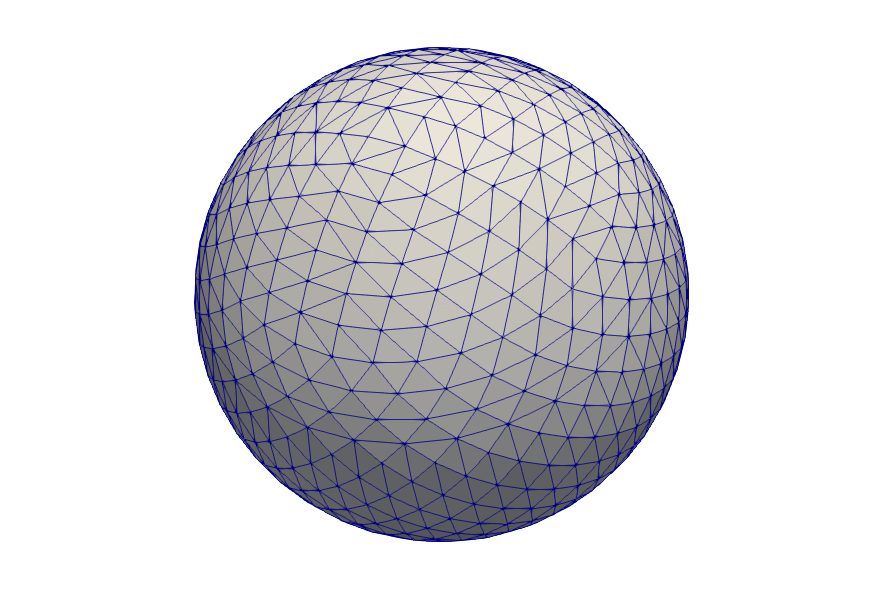
\includegraphics[width=0.4\textwidth]{figs/Chapter3/sphere_mesh.png}
	\end{center}
	\caption{\label{fig:sphere mesh}A triangulation $\mathcal T_h$ of the sphere made with the nodes of the HEALPix sampling with $N_{side}=8$}
\end{figure}

Taken any triangulation of the sphere $\mathcal T_h$, since $\mathbb S^2$ does not have boundaries and thus there are no boundary conditions to impose, this time the correct space $V_h$ to chose is $X^1_h$. The number of degrees of freedom of the space - and thus the number of basis functions - is equal to the number of vertices of the mesh and thanks to equation \ref{eq:dof and values} the solution $\mathbf f$ that is the vector of the coefficients of the function $f_h$ in the basis $\phi_i$ corresponds exactly to the values of the function $f_h$ in the vertices. For these reasons, the matrix $\mathbf L$ that we are looking for to perform our graph-like convolution is exactly
$$
\mathbf L = B^{-1}A
$$
However, having chosen a basis $\{\phi_i\}_i$ not orthonormal, $B$ is different to the identity matrix and its inverse is full, making $\mathbf L$ not adapt to perform graph-like convolutions. However this is a well known problem in the FEM literature; a common workaround is the so called \textit{lumping} of the mass matrix, that consist in replacing the matrix $B$ with the \textit{lumped} diagonal matrix $D$ obtained by placing in each diagonal entry $(D)_{ii}$ the sum of the elements of the i-th row of the mass matrix $B$:

\begin{equation}\label{eq:lumping}
D = \text{diag}\{d_i\},\quad d_i = \sum_j (B)_{ij}
\end{equation}

This approximation is well studied in literature and it is proved to work well in many practical cases. The inverse of the lumped mass matrix is diagonal as well $D^{-1} = \text{diag}\{\frac{1}{d_i}\}$ and thus the matrix $D^{-1}A$ in the lumped eigenvalue problem 
\begin{equation}\label{eq:lumped eigenvalue problem}
	D^{-1}A\mathbf f = \lambda \mathbf f
\end{equation}
has the same sparsity pattern of the stiffness matrix $A$, and thus leads to an acceptable computational cost of the filtering operation. However, $D^{-1}A$ is not symmetric; we then tried to use the symmetric matrix $\mathbf L = D^{-1/2}AD^{-1/2}$, thus solving the problem 
\begin{equation}\label{eq:symmetric lumped eigenvalue problem}
D^{-1/2}AD^{-1/2}\mathbf f = \lambda \mathbf f
\end{equation}
obtaining very promising results.
We implemented the eigenvalue problem \ref{eq:weak eigenvalue problem} in $X_h^1$. We show in figures \ref{fig:FEMHealpix}, \ref{fig:FEMequiangular} the usual analysis of the alignment of the eigenmodes for both HEALPix sampling and the equiangular sampling. Being the sphere convex, in both cases the mesh $\mathcal T_h$ has been obtained by calculating the triangulation of the convex hull of the nodes through the Qhull algorithm \cite{Barber96thequickhull}.

\begin{minipage}[t!]{.49\textwidth}
	\raggedleft
	\center
	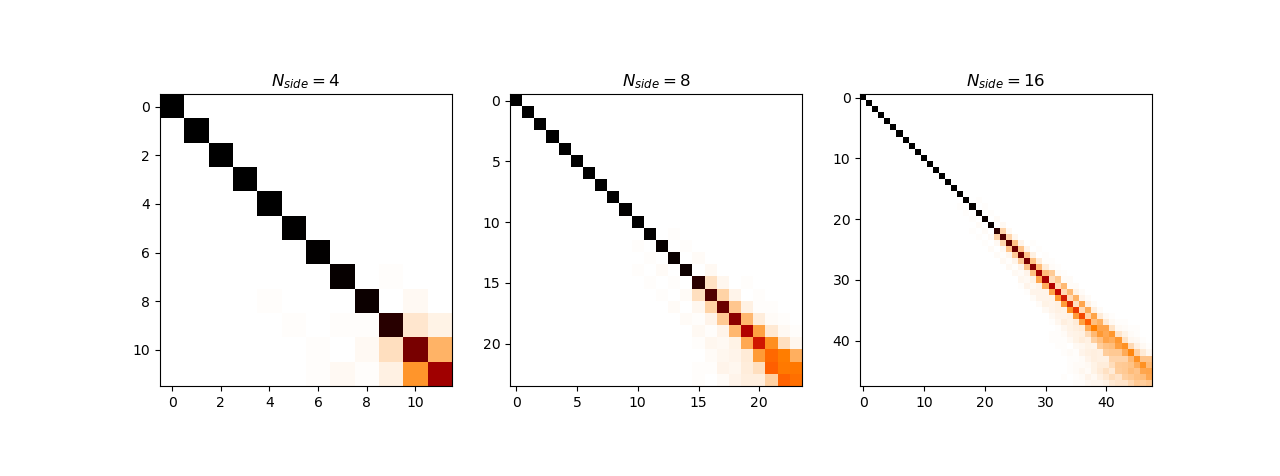
\includegraphics[width=0.9\linewidth]{../codes/03.FEM_laplacian/HEALPix/img/linearFEM.png}\\
	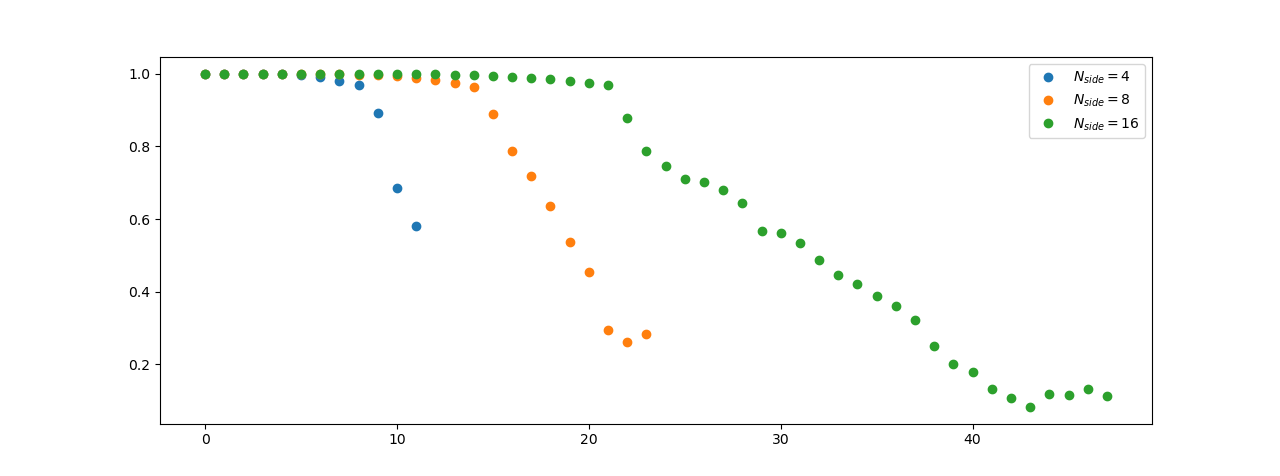
\includegraphics[width=0.9\linewidth]{../codes/03.FEM_laplacian/HEALPix/img/linearFEM_diagonal.png}	\\
	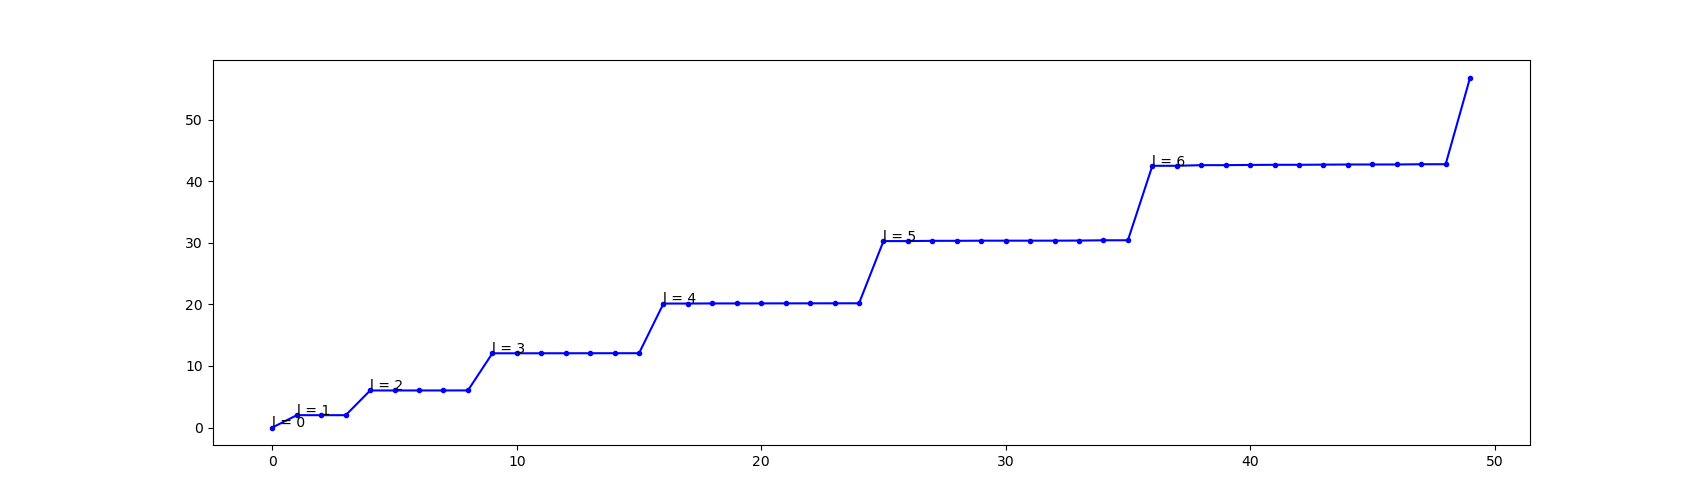
\includegraphics[width=0.9\linewidth]{../codes/03.FEM_laplacian/HEALPix/img/FEM_eigenvalues_16.png}	\\
	\captionof{figure}{	\label{fig:FEMHealpix}Alignment of eigenspaces using the linear FEM approximation to solve the eigenvalue problem \ref{eq:algebraic  eigenvalue problem} on HEALPix}

\end{minipage}
\hfill
%
\begin{minipage}[t!]{.49\textwidth}
	\raggedright
	\center
	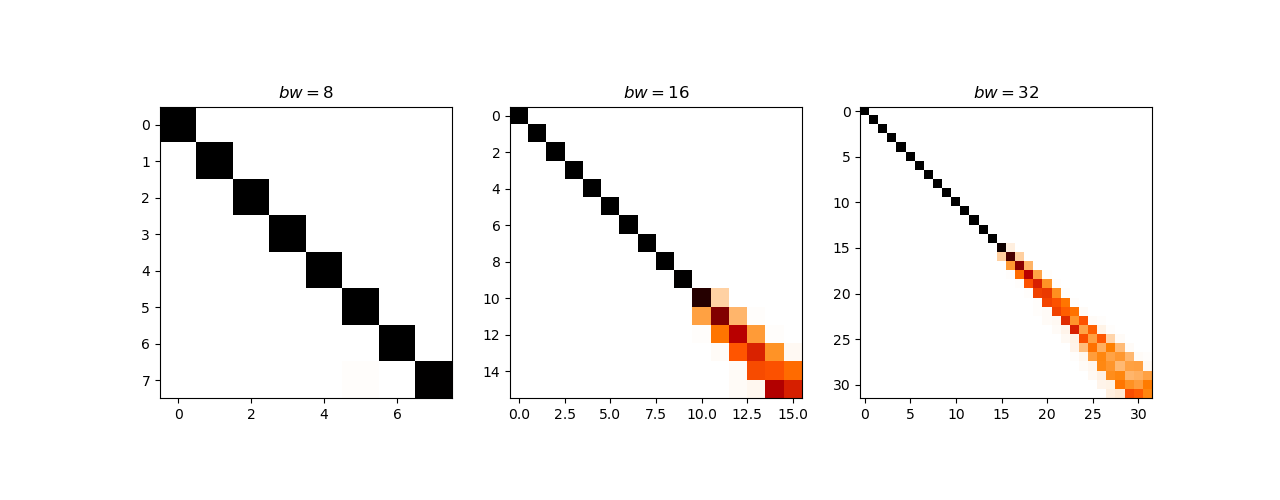
\includegraphics[width=0.9\linewidth]{../codes/03.FEM_laplacian/equiangular/normal/img/linearFEM.png}
	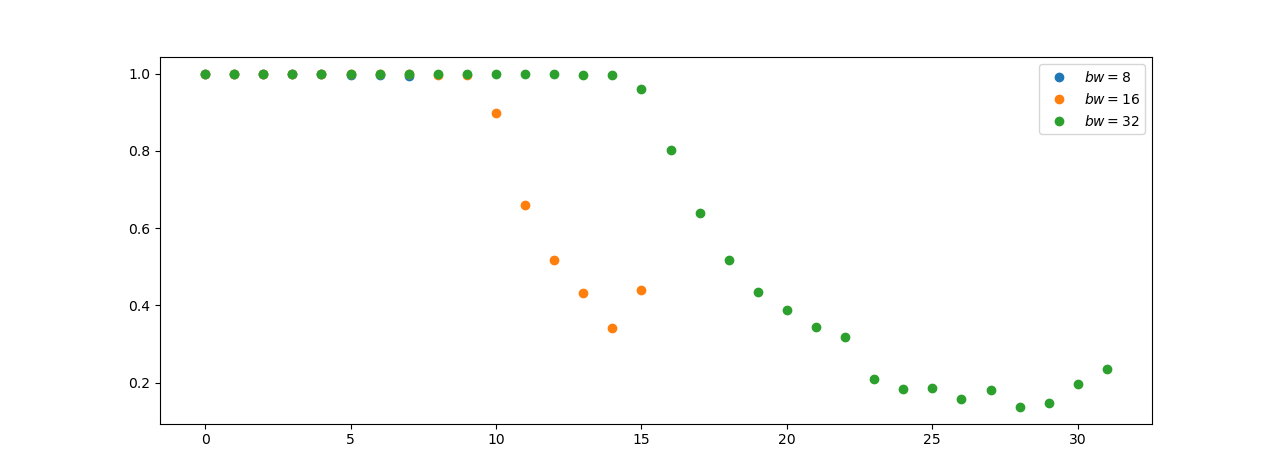
\includegraphics[width=0.9\linewidth]{../codes/03.FEM_laplacian/equiangular/normal/img/linearFEM_diagonal.png}	
	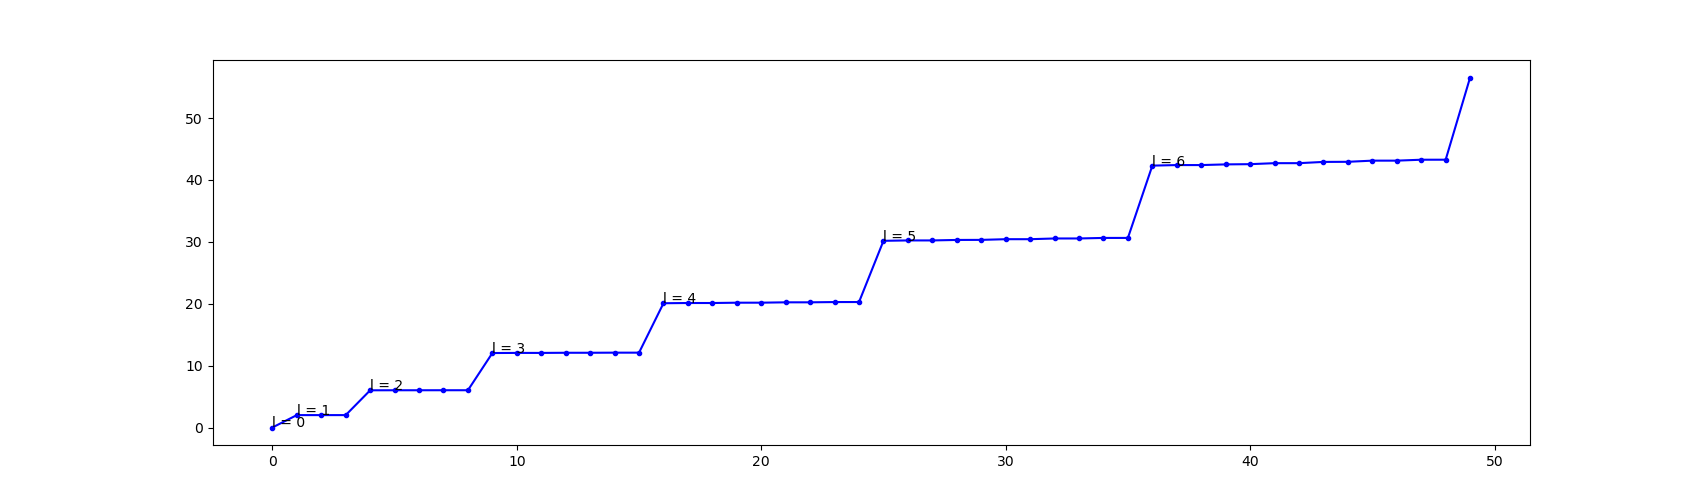
\includegraphics[width=0.9\linewidth]{../codes/03.FEM_laplacian/equiangular/normal/img/FEM_eigenvalues_16.png}	
	\captionof{figure}{\label{fig:FEMequiangular}Alignment of eigenspaces using the linear FEM approximation to solve the eigenvalue problem \ref{eq:algebraic  eigenvalue problem} on the equiangular sampling}
\end{minipage}
\begin{minipage}[t!]{.49\textwidth}
	\raggedleft
	\center
	\centering
	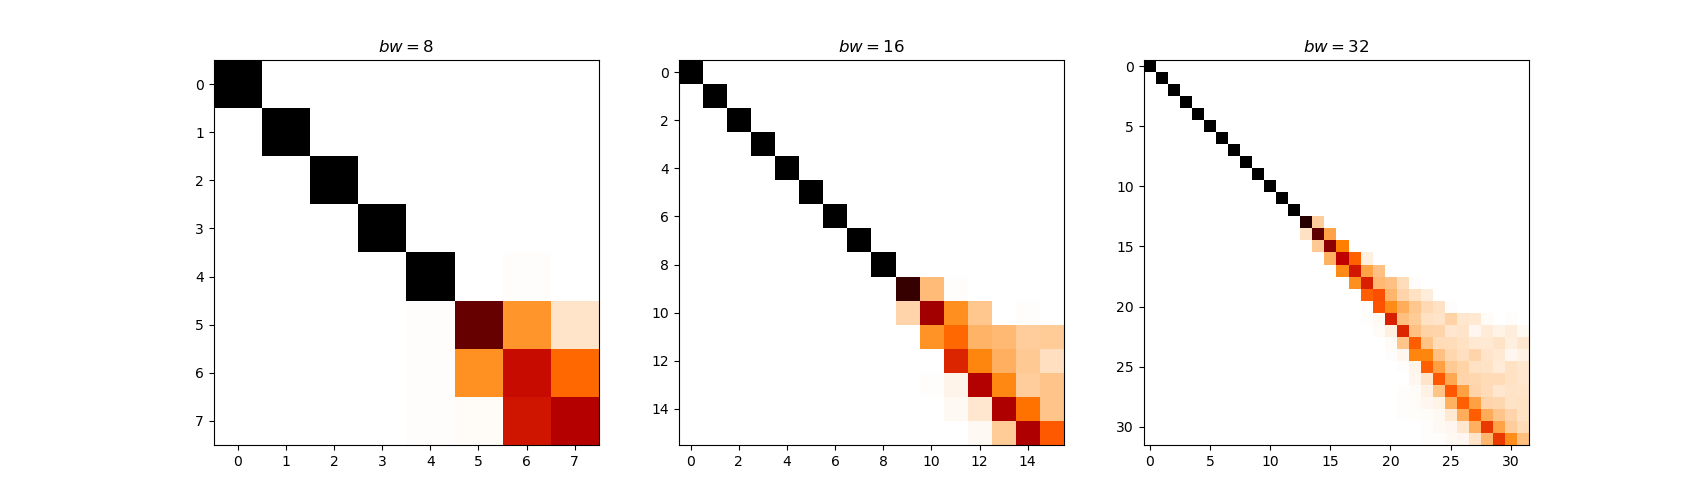
\includegraphics[width=0.9\textwidth]{../codes/03.FEM_laplacian/equiangular/mass_lumping/BL/img/linearFEM.png}
	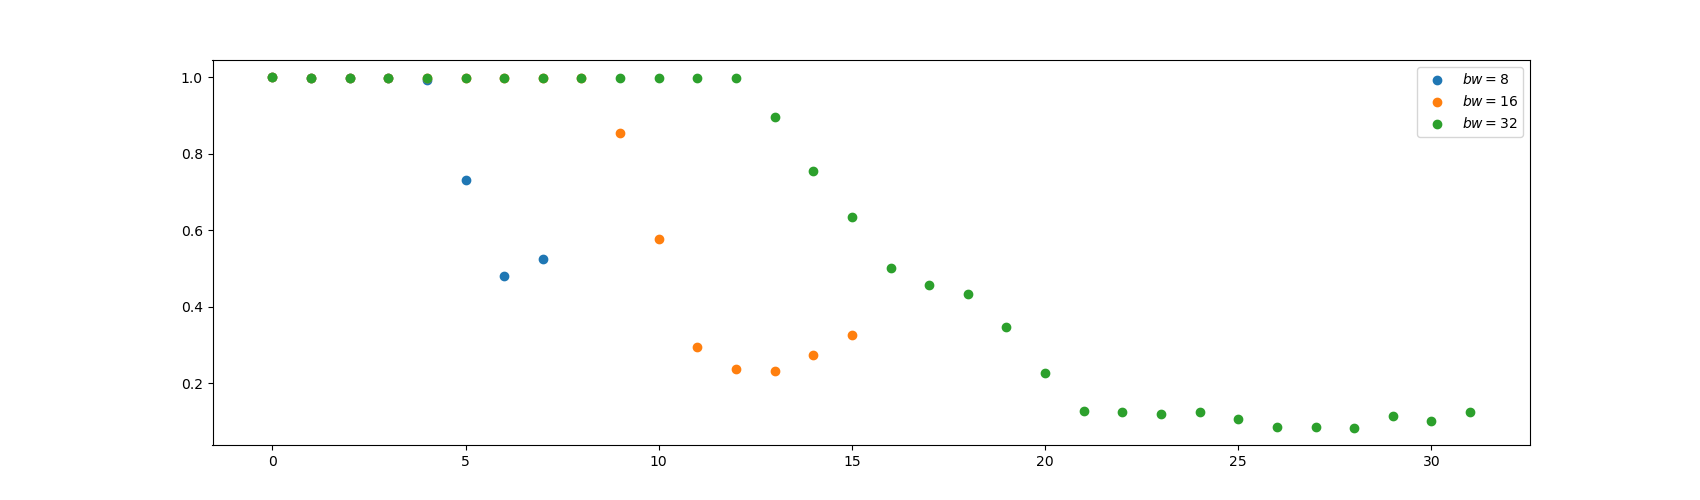
\includegraphics[width=0.9\textwidth]{../codes/03.FEM_laplacian/equiangular/mass_lumping/BL/img/linearFEM_diagonal.png}	
	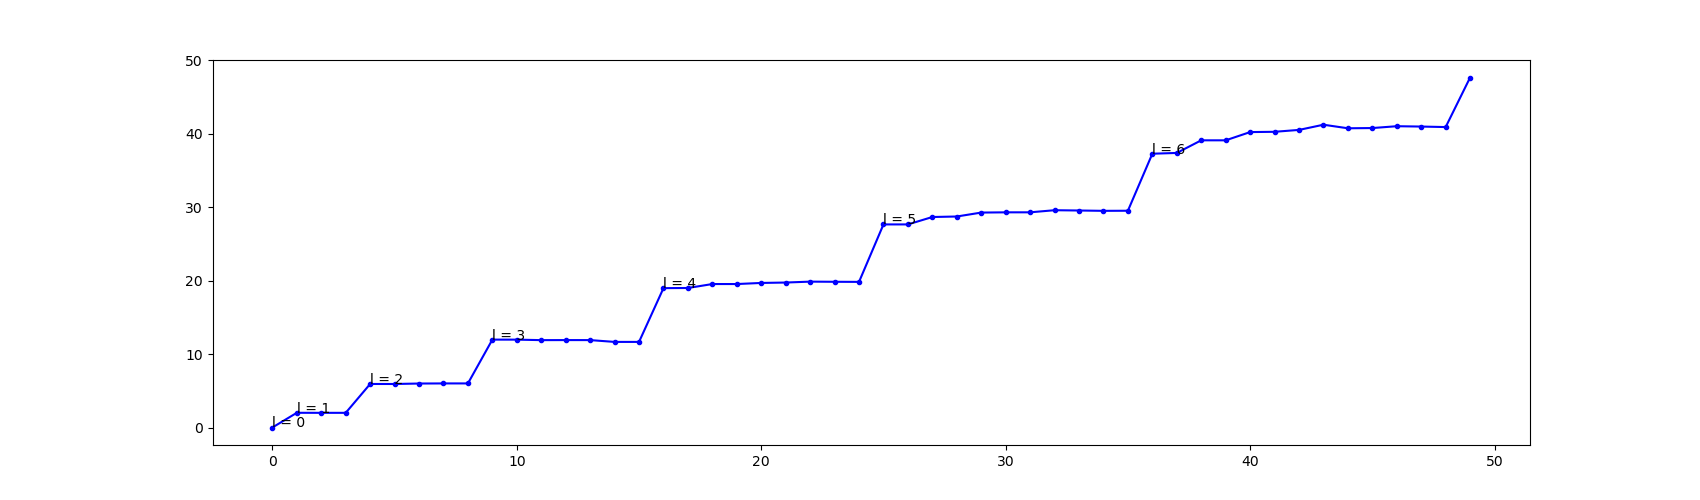
\includegraphics[width=0.9\textwidth]{../codes/03.FEM_laplacian/equiangular/mass_lumping/BL/img/FEM_eigenvalues_32.png}	
	\captionof{figure}{\label{fig:FEMequiangularLumped}Alignment of eigenspaces using the linear FEM approximation to solve the \textit{lumped} eigenvalue problem \ref{eq:lumped eigenvalue problem} on the equiangular sampling}
\end{minipage}
\hfill
%
\begin{minipage}[t!]{.49\textwidth}
	\raggedright
	\center
	\centering
	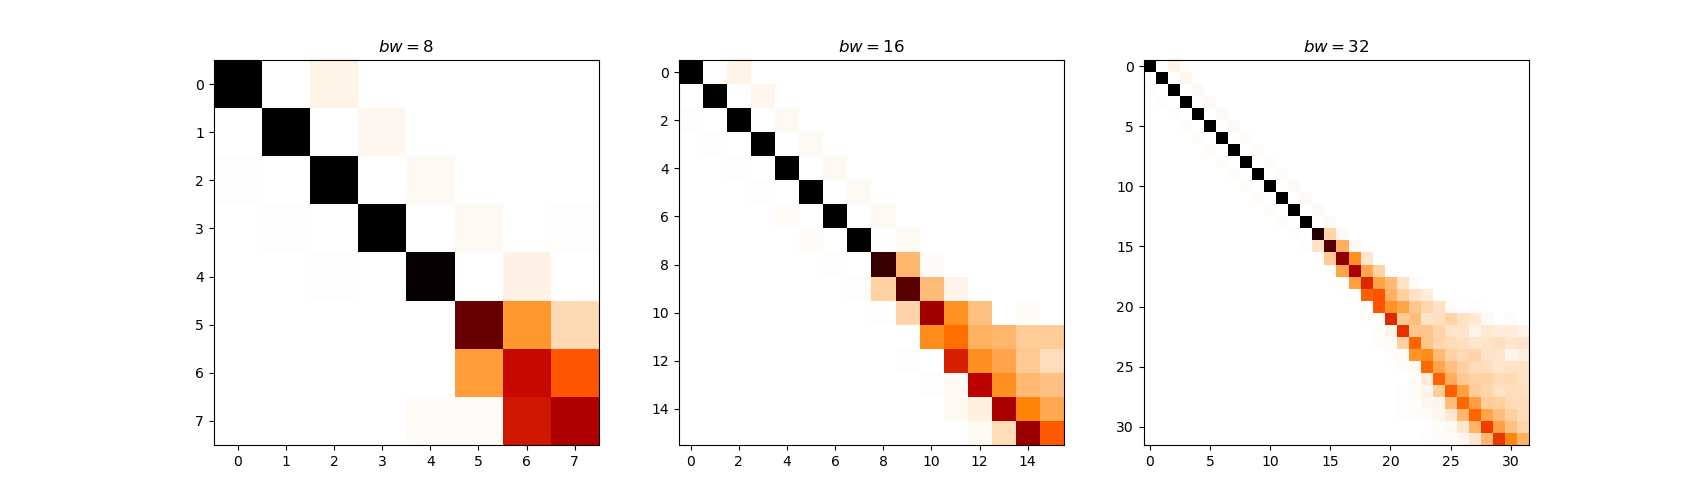
\includegraphics[width=0.9\textwidth]{../codes/03.FEM_laplacian/equiangular/mass_lumping/BLB/img/linearFEM.png}
	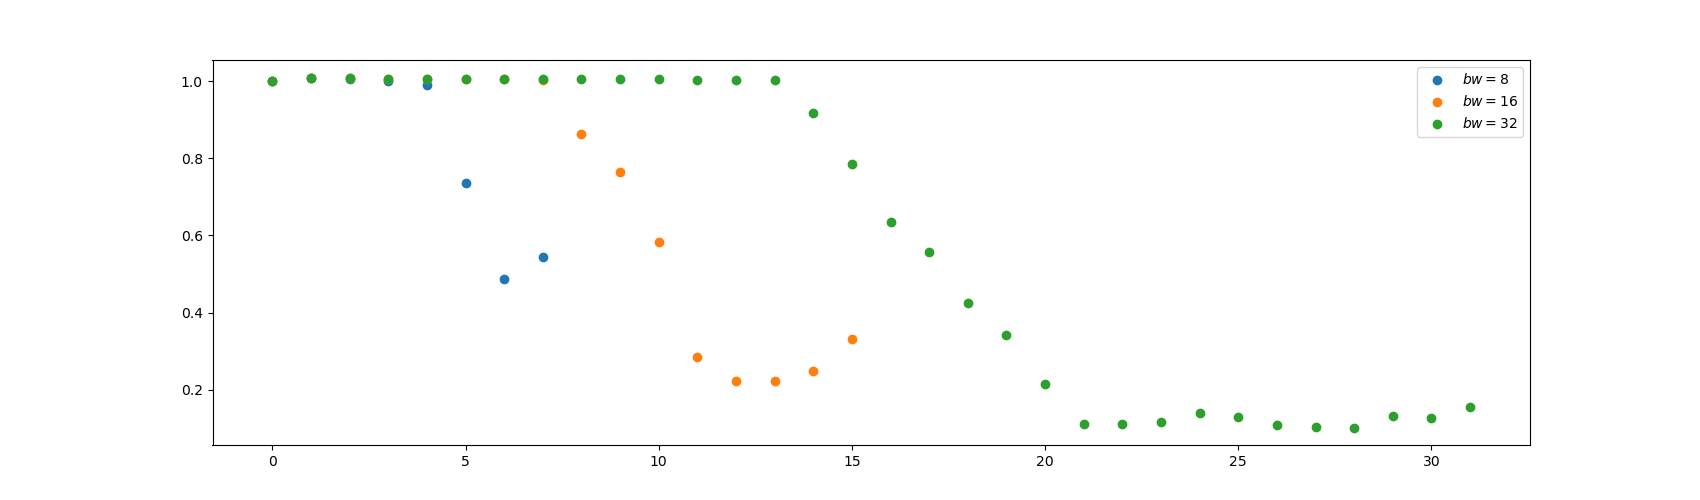
\includegraphics[width=0.9\textwidth]{../codes/03.FEM_laplacian/equiangular/mass_lumping/BLB/img/linearFEM_diagonal.png}	
	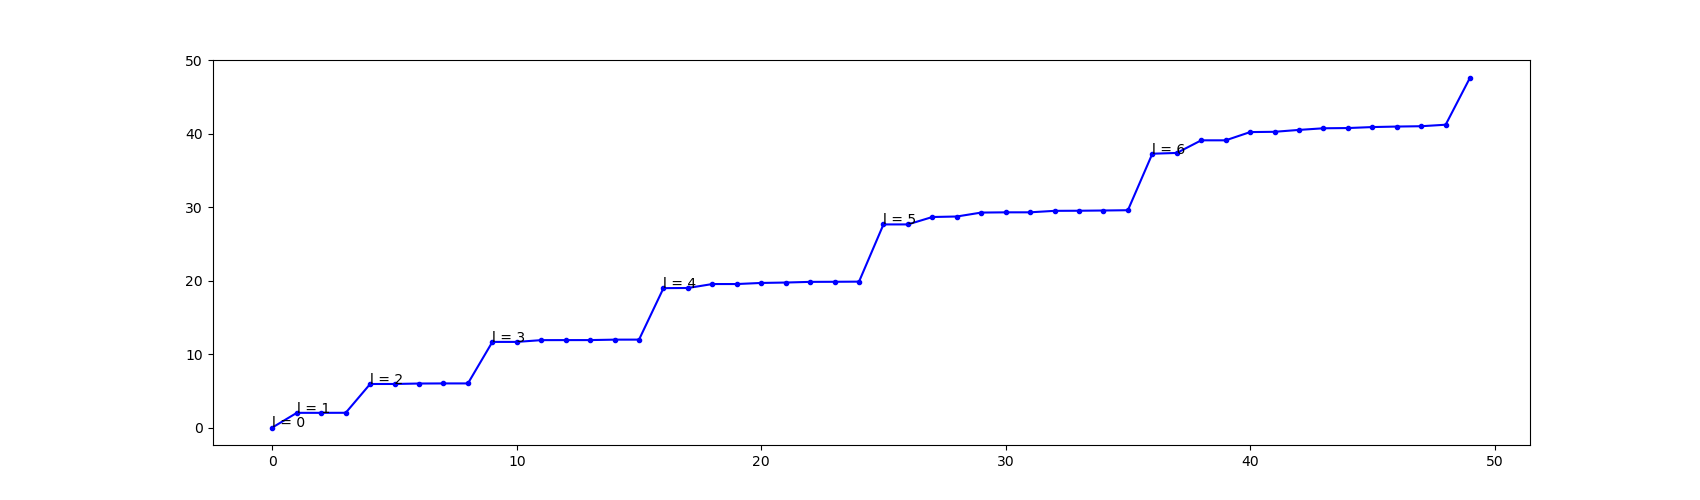
\includegraphics[width=0.9\textwidth]{../codes/03.FEM_laplacian/equiangular/mass_lumping/BLB/img/FEM_eigenvalues_32.png}	
	\captionof{figure}{\label{fig:symmetricFEMequiangularLumped}Alignment of eigenspaces using the linear FEM approximation to solve the \textit{symmetric lumped} eigenvalue problem \ref{eq:symmetric lumped eigenvalue problem} on the equiangular sampling}
\end{minipage}

We see that on HEALPix the \textit{full} HKGL shows better aligned eigenmodes than the \textit{full} FEM Laplacian $B^{-1}L$. On the equiangular sampling the FEM shows his capability of catching the geometry of the problem independently of the sampling (figure \ref{fig:FEMequiangular}). Furthermore it can be seen how on the equiangular sampling the solutions of the lumped problem \ref{eq:lumped eigenvalue problem } - figure \ref{fig:FEMequiangularLumped} - and of the symmetric lumped problem \ref{eq:symmetric lumped eigenvalue problem} - figure \ref{fig:symmetricFEMequiangularLumped} - look very close to the correct solution of the problem \ref{eq:algebraic  eigenvalue problem}, thus making the FEM approach very promising.



\subsubsection{Diffusion with the exponential matrix}

To show that it is possible to filter a signal with the matrix $\mathbf L = D^{-1/2}AD^{-1/2}$ in the graph-like way and to confront it to the full HKGL with tried to filter a signal concentrated on a node  with the well known diffusion filter $\exp{-\tau \mathbf L}$. To enhance the deformation caused by the HKGL it was chosen a very irregular sampling shown in figure \ref{fig:FEM lumped symmetric diffusion on irregular sampling}. It can be seen how the full HKGL compresses the signal around the equator where the sampling is more sparse; the FEM filtering manages to keep the diffusion homogeneous no matter the asymmetry in the sampling. 
\begin{figure}[h]
	
	\centering
	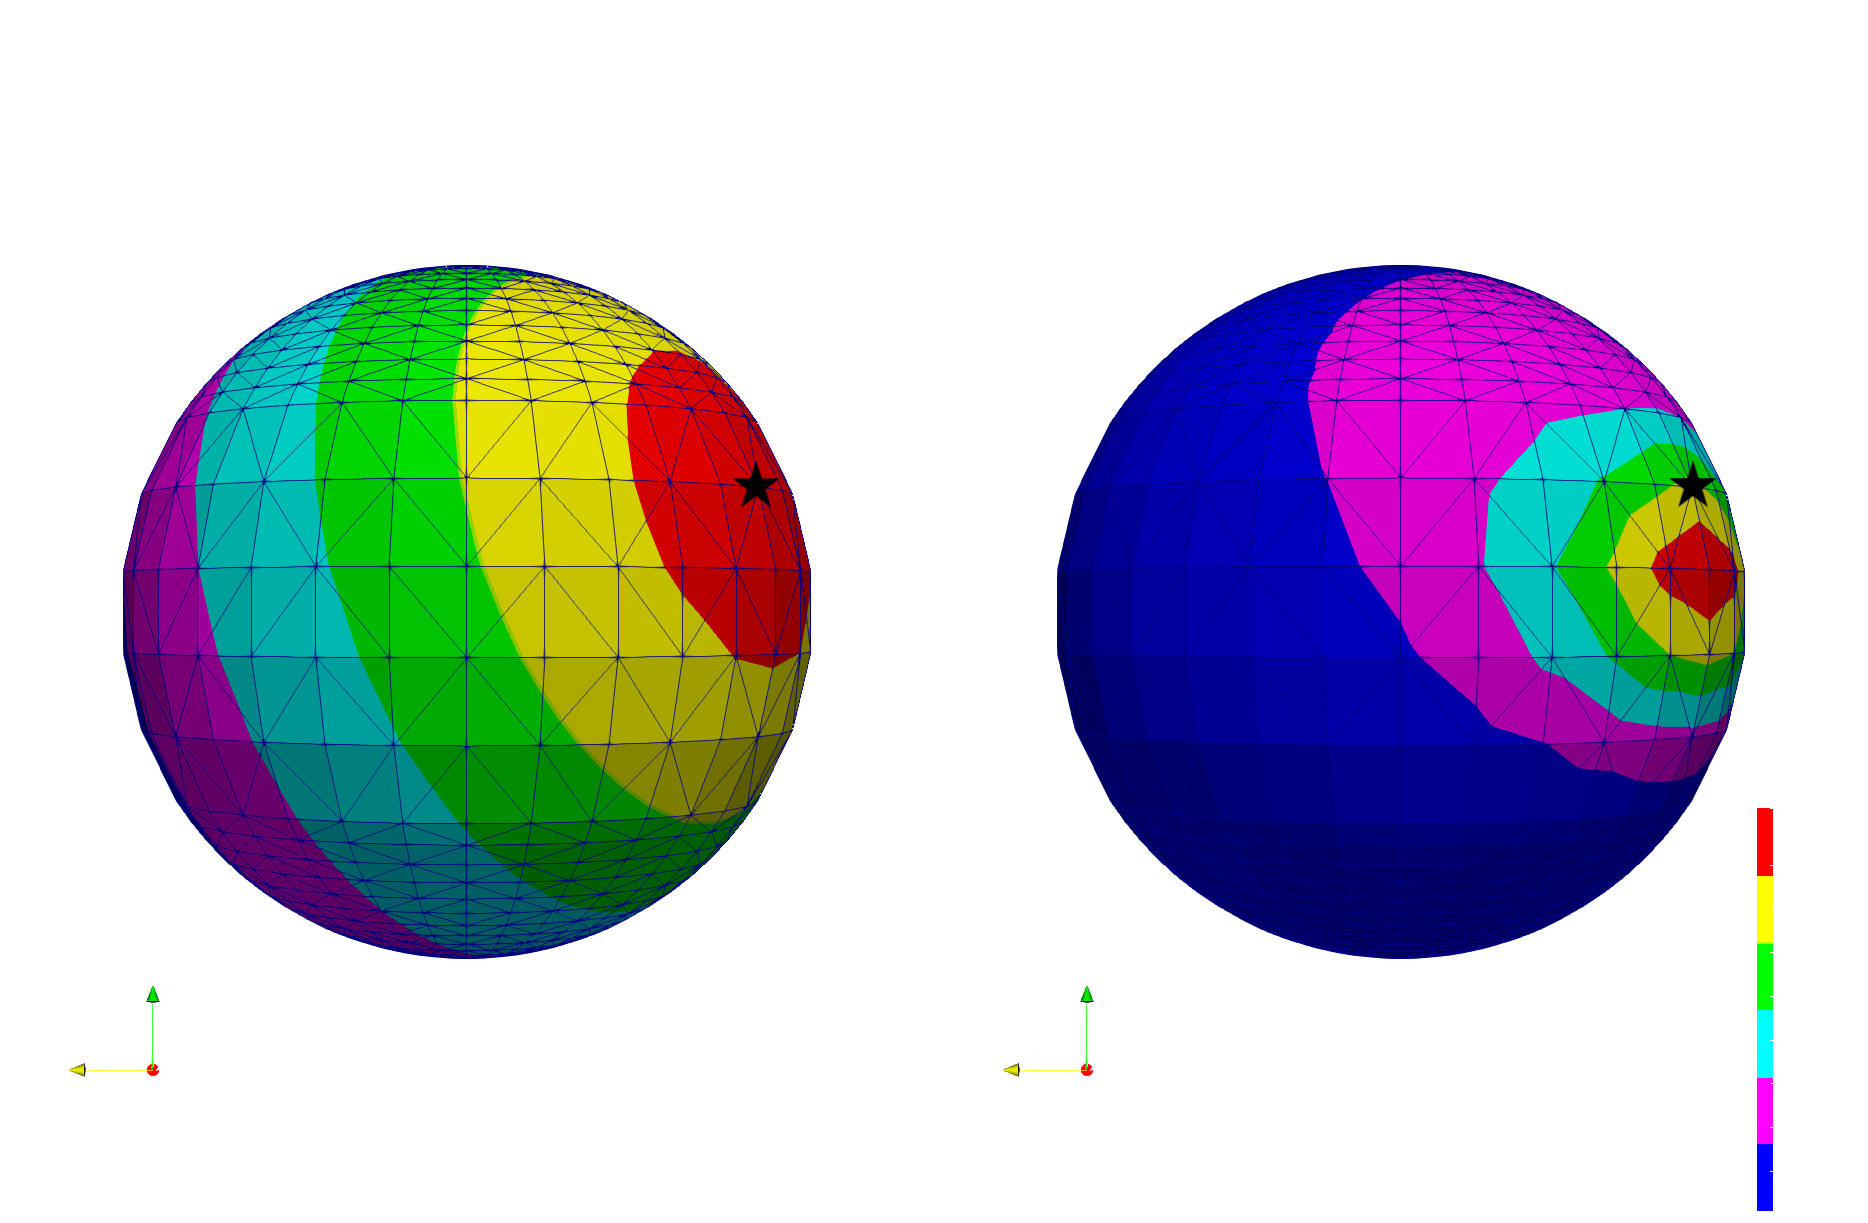
\includegraphics[width=0.8\textwidth]{figs/Chapter3/diffusion.png}
	\caption{\label{fig:FEM lumped symmetric diffusion on irregular sampling}Symmetric lumped linear FEM diffusion and HKGL diffusion on an irregular sampling of the sphere. The position of the filtered source signal is indicated with a black star.}
\end{figure}






